% Options for packages loaded elsewhere
\PassOptionsToPackage{unicode}{hyperref}
\PassOptionsToPackage{hyphens}{url}
%
\documentclass[
  ignorenonframetext,
  serif,
  professionalfont,
  usenames,
  dvipsnames,
  aspectratio = 169]{beamer}
\usepackage{pgfpages}
\setbeamertemplate{caption}[numbered]
\setbeamertemplate{caption label separator}{: }
\setbeamercolor{caption name}{fg=normal text.fg}
\beamertemplatenavigationsymbolsempty
% Prevent slide breaks in the middle of a paragraph
\widowpenalties 1 10000
\raggedbottom
\setbeamertemplate{part page}{
  \centering
  \begin{beamercolorbox}[sep=16pt,center]{part title}
    \usebeamerfont{part title}\insertpart\par
  \end{beamercolorbox}
}
\setbeamertemplate{section page}{
  \centering
  \begin{beamercolorbox}[sep=12pt,center]{part title}
    \usebeamerfont{section title}\insertsection\par
  \end{beamercolorbox}
}
\setbeamertemplate{subsection page}{
  \centering
  \begin{beamercolorbox}[sep=8pt,center]{part title}
    \usebeamerfont{subsection title}\insertsubsection\par
  \end{beamercolorbox}
}
\AtBeginPart{
  \frame{\partpage}
}
\AtBeginSection{
  \ifbibliography
  \else
    \frame{\sectionpage}
  \fi
}
\AtBeginSubsection{
  \frame{\subsectionpage}
}
\usepackage{amsmath,amssymb}
\usepackage{lmodern}
\usepackage{iftex}
\ifPDFTeX
  \usepackage[T1]{fontenc}
  \usepackage[utf8]{inputenc}
  \usepackage{textcomp} % provide euro and other symbols
\else % if luatex or xetex
  \usepackage{unicode-math}
  \defaultfontfeatures{Scale=MatchLowercase}
  \defaultfontfeatures[\rmfamily]{Ligatures=TeX,Scale=1}
\fi
% Use upquote if available, for straight quotes in verbatim environments
\IfFileExists{upquote.sty}{\usepackage{upquote}}{}
\IfFileExists{microtype.sty}{% use microtype if available
  \usepackage[]{microtype}
  \UseMicrotypeSet[protrusion]{basicmath} % disable protrusion for tt fonts
}{}
\makeatletter
\@ifundefined{KOMAClassName}{% if non-KOMA class
  \IfFileExists{parskip.sty}{%
    \usepackage{parskip}
  }{% else
    \setlength{\parindent}{0pt}
    \setlength{\parskip}{6pt plus 2pt minus 1pt}}
}{% if KOMA class
  \KOMAoptions{parskip=half}}
\makeatother
\usepackage{xcolor}
\IfFileExists{xurl.sty}{\usepackage{xurl}}{} % add URL line breaks if available
\IfFileExists{bookmark.sty}{\usepackage{bookmark}}{\usepackage{hyperref}}
\hypersetup{
  pdfauthor={Lineu Alberto Cavazani de Freitas; Orientador: Prof.~Dr.~Wagner Hugo Bonat},
  pdflang={pt-BR},
  hidelinks,
  pdfcreator={LaTeX via pandoc}}
\urlstyle{same} % disable monospaced font for URLs
\newif\ifbibliography
\usepackage{graphicx}
\makeatletter
\def\maxwidth{\ifdim\Gin@nat@width>\linewidth\linewidth\else\Gin@nat@width\fi}
\def\maxheight{\ifdim\Gin@nat@height>\textheight\textheight\else\Gin@nat@height\fi}
\makeatother
% Scale images if necessary, so that they will not overflow the page
% margins by default, and it is still possible to overwrite the defaults
% using explicit options in \includegraphics[width, height, ...]{}
\setkeys{Gin}{width=\maxwidth,height=\maxheight,keepaspectratio}
% Set default figure placement to htbp
\makeatletter
\def\fps@figure{htbp}
\makeatother
\setlength{\emergencystretch}{3em} % prevent overfull lines
\providecommand{\tightlist}{%
  \setlength{\itemsep}{0pt}\setlength{\parskip}{0pt}}
\setcounter{secnumdepth}{-\maxdimen} % remove section numbering
\ifLuaTeX
\usepackage[bidi=basic]{babel}
\else
\usepackage[bidi=default]{babel}
\fi
\babelprovide[main,import]{brazilian}
% get rid of language-specific shorthands (see #6817):
\let\LanguageShortHands\languageshorthands
\def\languageshorthands#1{}
% Definição do esquema de cores:
% 1. UFPR - Azul com cinza.
% 2. DEST - Roxo com cinza.
% 3. LEG - Laranjado com cinza.
\def\mycolorscheme{1}

% Caminho para a imagem de fundo com aspecto 16x9.
% \def\pathtobg{config/ufpr-fachada-baixo-1.jpg}
% \def\pathtobg{config/ufpr-fundo.jpg}
% \def\pathtobg{config/ufpr-fundo.jpg}
\def\pathtobg{./config/ufpr-fundo-16x9.jpg}

% \providecommand{\tightlist}{%
%   \setlength{\itemsep}{0pt}\setlength{\parskip}{0pt}}
% ATTENTION: Redefine o comando acima que é definido pelo template.
% \renewcommand{\tightlist}{}
\renewcommand{\tightlist}{%
  \setlength{\itemsep}{0\baselineskip}
  \setlength{\parskip}{0.25\baselineskip}
}

% Logo na capa.
\titlegraphic{
  \vspace{-2em}
  
\includegraphics[height=1.8cm]{config/capes_tp2.png}\hspace{1em}
  
\includegraphics[height=1.8cm]{config/ufpr-transparent-600px.png}\hspace{1em}
  
\includegraphics[height=1.8cm]{config/dsbd-2x2-trans.png}
}
%-----------------------------------------------------------------------

% Palladio.
% \usepackage[sc]{mathpazo}
% \linespread{1.05}         % Palladio needs more leading (space between lines)
% \usepackage[T1]{fontenc}

% Kurier.
% \usepackage[light, condensed, math]{kurier}
% \usepackage[T1]{fontenc}

% Iwona.
% \usepackage[math, light, condensed]{iwona}

% \usepackage{cmbright}
% \usepackage[charter]{mathdesign}
% \usepackage{palatino}

% Roboto (with Iwona for maths).
% \usepackage[math]{iwona}
% \usepackage[sfdefault, light, condensed]{roboto}

% Source Sans Pro (with Iwona for maths).
% \usepackage[math]{iwona}
% \usepackage[default, light]{sourcesanspro}

% Lato (with Iwona for maths).
% \usepackage[math]{iwona}
% \usepackage[default]{lato}

% Fira Sans (with Iwona for maths).
\usepackage[math, light]{iwona}
\usepackage[sfdefault,light]{FiraSans} %% option 'sfdefault' activates Fira Sans as the default text font
\usepackage[T1]{fontenc}
\renewcommand*\oldstylenums[1]{{\firaoldstyle #1}}

% Font for code. ----------------------------
% \usepackage[scaled=.75]{beramono}
\usepackage{inconsolata}

% ATTENTION: needs complile with xelatex: `$ xelatex file.tex`
% \usepackage{fontspec}
% \setmonofont{M+ 1m}
% \setmonofont{M+ 1mn}
% \setmonofont{M+ 2m}

%-----------------------------------------------------------------------

% \usepackage{lmodern}
\usepackage{amssymb, amsmath}
\usepackage[makeroom]{cancel}
% \usepackage{ifxetex, ifluatex}
\usepackage{fixltx2e} % provides \textsubscript
\usepackage[utf8]{inputenc}
%\usepackage[shorthands=off,main=brazil]{babel}
\usepackage{graphicx}
\usepackage{xcolor}
\usepackage{setspace}
\usepackage{comment}
\usepackage{icomma}

%-----------------------------------------------------------------------
% Algumas configurações.

\setlength{\parindent}{0pt}
\setlength{\parskip}{6pt plus 2pt minus 1pt}
\setlength{\emergencystretch}{3em}  % prevent overfull lines
% \providecommand{\tightlist}{%
%   \setlength{\itemsep}{0pt}\setlength{\parskip}{0pt}}
\setcounter{secnumdepth}{0}

% Espaço vertical para o ambiente `quote`.
\let\oldquote\quote
\let\oldendquote\endquote
\renewenvironment{quote}{%
  \vspace{1em}\oldquote}{%
  \oldendquote\vspace{1em}}

%-----------------------------------------------------------------------
% Espaçamento entre items para itemize, enumerate e description.

% % itemize.
% \let\itemopen\itemize
% \let\itemclose\enditemize
% \renewenvironment{itemize}{%
%   \itemopen\addtolength{\itemsep}{0.25\baselineskip}}{\itemclose}
%
% % enumerate.
% \let\enumopen\enumerate
% \let\enumclose\endenumerate
% \renewenvironment{enumerate}{%
%   \enumopen\addtolength{\itemsep}{0.25\baselineskip}}{\enumclose}
%
% % description.
% \let\descopen\description
% \let\descclose\enddescription
% \renewenvironment{description}{%
%   \descopen\addtolength{\itemsep}{0.25\baselineskip}}{\descclose}

%-----------------------------------------------------------------------

% \usepackage[hang]{caption}
\usepackage{caption}
\captionsetup{font=footnotesize,
  labelfont={color=mycolor1, footnotesize},
  labelsep=period}

% \providecommand{\tightlist}{%
%   \setlength{\itemsep}{0pt}\setlength{\parskip}{0pt}}

%-----------------------------------------------------------------------

\usepackage{tikz}
\usepackage{pgfplots}
\usepackage{multirow}

% \def\pathtobg{/home/walmes/Projects/templates/COMMON/ufpr-fundo.jpg}
% \def\pathtobg{/home/walmes/Projects/templates/COMMON/ufpr-fundo-16x9.jpg}
% \def\pathtobg{/home/walmes/Projects/templates/COMMON/ufpr-fachada-dir-1.jpg}
% \def\pathtobg{/home/walmes/Projects/templates/COMMON/ufpr-fachada-esq-1.jpg}
% \def\pathtobg{/home/walmes/Projects/templates/COMMON/ufpr-perto-1.jpg}
% \def\pathtobg{/home/walmes/Projects/templates/COMMON/ufpr-fachada-baixo-1.jpg}

\ifx\pathtobg\undefined
\else
  \usebackgroundtemplate{
    \tikz[overlay, remember picture]
    \node[% opacity=0.3,
          at=(current page.south east),
          anchor=south east,
          inner sep=0pt] {
            \includegraphics[height=\paperheight, width=\paperwidth]{\pathtobg}};
  }
\fi

%-----------------------------------------------------------------------
% Definições de esquema de cores.

\ifx\mycolorscheme\undefined
  % UFPR.
  % http://www.color-hex.com/color-palette/2018
  \definecolor{mycolor1}{HTML}{015c93} % Título.
  \definecolor{mycolor2}{HTML}{363435} % Texto.
  \definecolor{mycolor3}{HTML}{015c93} % Estrutura.
  \definecolor{mycolor4}{HTML}{015c93} % Links.
  \definecolor{mycolor5}{HTML}{CECAC5} % Preenchimentos.
\else
  \if\mycolorscheme1
    % UFPR.
    \definecolor{mycolor1}{HTML}{015c93} % Título.
    \definecolor{mycolor2}{HTML}{363435} % Texto.
    \definecolor{mycolor3}{HTML}{015c93} % Estrutura.
    \definecolor{mycolor4}{HTML}{015c93} % Links.
    \definecolor{mycolor5}{HTML}{CECAC5} % Preenchimentos.
  \fi
  \if\mycolorscheme2
    % DEST.
    \definecolor{mycolor1}{HTML}{2a0e72} % Título.
    \definecolor{mycolor2}{HTML}{202E35} % Texto.
    \definecolor{mycolor3}{HTML}{2a0e72} % Estrutura.
    % \definecolor{mycolor3}{HTML}{8072a3} % Estrutura.
    \definecolor{mycolor4}{HTML}{2a0e72} % Links.
    % \definecolor{mycolor4}{HTML}{bfb9d1} % Links.
    % \definecolor{mycolor5}{HTML}{AEA79F} % Preenchimentos.
    \definecolor{mycolor5}{HTML}{CECAC5} % Preenchimentos.
  \fi
  \if\mycolorscheme3
    % LEG.
    \definecolor{mycolor2}{HTML}{363435} % Texto.
    % \definecolor{mycolor1}{HTML}{ff8000} % Título.
    % \definecolor{mycolor3}{HTML}{ff8000} % Estrutura.
    % \definecolor{mycolor4}{HTML}{ff8000} % Links.
    % \definecolor{mycolor1}{HTML}{E57300} % Título.
    % \definecolor{mycolor3}{HTML}{E57300} % Estrutura.
    % \definecolor{mycolor4}{HTML}{E57300} % Links.
    \definecolor{mycolor1}{HTML}{F67014} % Título.
    \definecolor{mycolor3}{HTML}{F67014} % Estrutura.
    \definecolor{mycolor4}{HTML}{F67014} % Links.
    % \definecolor{mycolor1}{HTML}{FE5C23} % Título.
    % \definecolor{mycolor3}{HTML}{FE5C23} % Estrutura.
    % \definecolor{mycolor4}{HTML}{FE5C23} % Links.
    \definecolor{mycolor5}{HTML}{222222} % Preenchimentos.
    \definecolor{mycolor5}{HTML}{383838} % Preenchimentos.
  \fi
\fi

\hypersetup{
  colorlinks=true,
  linkcolor=mycolor4,
  urlcolor=mycolor1,
  citecolor=mycolor1
}

%-----------------------------------------------------------------------
% ATTENTION: http://www.cpt.univ-mrs.fr/~masson/latex/Beamer-appearance-cheat-sheet.pdf

\usetheme{Boadilla}
\usecolortheme{default}

% \setbeamersize{text margin left=7mm, text margin right=7mm}
% \setbeamertemplate{frametitle}[default][left, leftskip=3mm]
% \addtobeamertemplate{frametitle}{\vspace{0.5em}}{}

\setbeamertemplate{caption}[numbered]
\setbeamertemplate{section in toc}[sections numbered]
\setbeamertemplate{subsection in toc}[subsections numbered]
\setbeamertemplate{sections/subsections in toc}[ball]{}
\setbeamertemplate{sections in toc}[ball]
\setbeamercolor{section number projected}{bg=mycolor1, fg=white}
\setbeamertemplate{blocks}[rounded]
\setbeamertemplate{navigation symbols}{}
\setbeamertemplate{frametitle continuation}{\gdef\beamer@frametitle{}}
% \setbeamertemplate{frametitle}[default][center]
%\setbeamertemplate{footline}[frame number]

\setbeamerfont{page number in head/foot}{size=\large}

\setbeamertemplate{footline}{
  \hfill%
  \usebeamercolor[fg]{page number in head/foot}%
  \usebeamerfont{page number in head/foot}%
  \setbeamertemplate{page number in head/foot}[framenumber]%
  \usebeamertemplate*{page number in head/foot}\kern1em\vskip2pt%
}

\setbeamertemplate{enumerate items}[default]
\setbeamertemplate{itemize items}{\scriptsize\raise1.25pt\hbox{\donotcoloroutermaths$\blacktriangleright$}}

% Blocos.
% \addtobeamertemplate{block begin}{\vskip -\bigskipamount}{}
% \addtobeamertemplate{block end}{}{\vskip -\bigskipamount}
\addtobeamertemplate{block begin}{\vspace{0.5em}}{}
\addtobeamertemplate{block end}{}{\vspace{0.5em}}


% Rodapé.
\setbeamercolor{title in head/foot}{parent=subsection in head/foot}
\setbeamercolor{author in head/foot}{bg=mycolor4, fg=white}
\setbeamercolor{date in head/foot}{parent=subsection in head/foot, fg=mycolor3}

% Cabeçalho.
\setbeamercolor{section in head/foot}{bg=mycolor2, fg=mycolor4}
\setbeamercolor{subsection in head/foot}{bg=mycolor2, fg=white}

\setbeamercolor{title}{fg=mycolor1}       % Título dos slides.
\setbeamercolor{titlelike}{fg=title}
\setbeamercolor{subtitle}{fg=mycolor2}    % Subtítulo.
\setbeamercolor{institute in head/foot}{parent=palette primary} % Instituição.
\setbeamercolor{frametitle}{fg=mycolor1}  % De quadro.
\setbeamercolor{structure}{fg=mycolor3}   % Listas e rodapé.
\setbeamercolor{item projected}{bg=mycolor2}
\setbeamercolor{block title}{bg=mycolor5, fg=mycolor2}
\setbeamercolor{normal text}{fg=mycolor2} % Texto.
\setbeamercolor{caption name}{fg=normal text.fg}
% \setbeamercolor{footlinecolor}{fg=mycolor2, bg=mycolor5}
% \setbeamercolor{section in head/foot}{fg=mycolor2, bg=mycolor5}
\setbeamercolor{author in head/foot}{fg=white, bg=mycolor1}
\setbeamercolor{section in foot}{fg=mycolor4, bg=mycolor5}
\setbeamercolor{date in foot}{fg=mycolor4, bg=mycolor5}
\setbeamercolor{block title}{fg=white, bg=mycolor1}
\setbeamercolor{block body}{fg=black, bg=white!80!gray}
\setbeamercolor{block body}{fg=black, bg=white!80!gray}

% To remove empty brackets of \institution.
% \makeatletter
% \setbeamertemplate{footline}{
%   \leavevmode%
%   \hbox{%
%     \begin{beamercolorbox}[
%       wd=0.3\paperwidth, ht=2.25ex, dp=1ex, right]{author in head/foot}%
%       \usebeamerfont{author in head/foot}\insertshortauthor{}\hspace*{1ex}
%     \end{beamercolorbox}%
%     \begin{beamercolorbox}[
%       wd=0.6\paperwidth, ht=2.25ex, dp=1ex, left]{section in foot}%
%       \usebeamerfont{title in head/foot}\hspace*{1ex}\insertshorttitle{}
%       % \usebeamerfont{title in head/foot}\hspace*{1ex}\insertframetitle{}
%     \end{beamercolorbox}%
%     \begin{beamercolorbox}[
%       wd=0.1\paperwidth, ht=2.25ex, dp=1ex, right]{date in foot}%
%       \insertframenumber{}\hspace*{2ex}
%     \end{beamercolorbox}
%   }%
%   \vskip0pt%
% }
% \makeatother

%-----------------------------------------------------------------------

% \usepackage{hyphenat}
\usepackage{changepage}

% Slide para o título das seções.
\AtBeginSection[]{
  \begin{frame}
    % \vfill
    \vspace{4cm}
    % \centering
    % \begin{beamercolorbox}[sep = 8pt, center, shadow = true, rounded = true]{title}
    \begin{beamercolorbox}{title}
      \begin{columns}
        \column{0.7\linewidth}
        {\LARGE\textbf \insertsectionhead}
      \end{columns}
    \end{beamercolorbox}
    \vfill
  \end{frame}
}

%-----------------------------------------------------------------------
%---- preamble-chunk.tex -----------------------------------------------

% Knitr.

% ATTENTION: this needs `\usepackage{xcolor}'.
\definecolor{color_line}{HTML}{333333}
\definecolor{color_back}{HTML}{DDDDDD}
% \definecolor{color_back}{HTML}{FF0000}

% ATTENTION: usa o fancyvrb.
% https://ctan.math.illinois.edu/macros/latex/contrib/fancyvrb/doc/fancyvrb-doc.pdf
% R input.
\usepackage{tcolorbox}
\ifcsmacro{Highlighting}{
  % Statment if it exists. ------------------
  \DefineVerbatimEnvironment{Highlighting}{Verbatim}{
     %frame=lines,     % Linha superior e inferior.
     framesep=2ex,    % Distância da linha para o texto.
     framerule=0.5pt, % Espessura da linha.
    % rulecolor=\color{color_line},
    %numbers=right,
    fontsize=\footnotesize, % Tamanho da fonte.
    baselinestretch=1.2,   % Espaçamento entre linhas.
    commandchars=\\\{\}}
  % Margens do ambiente `Shaded'.
  % \fvset{listparameters={\setlength{\topsep}{-1em}}}
  % \renewenvironment{Shaded}{\vspace{-1ex}}{\vspace{-2ex}}
  %\renewenvironment{Shaded}{
  %  \vspace{2pt}
    %\begin{tcolorbox}[
%      boxrule=0pt,      % Espessura do contorno.
%      colframe=gray!10, % Cor do contorno.
      %colback=gray!10,  % Cor de fundo da caixa.
      % arc=1em,          % Raio para contornos arredondados.
      %sharp corners,
      % boxsep=0.5em,     % Margem interna.
      %left=3pt, right=3pt, top=3pt, bottom=3pt, % Margens internas.
      % grow to left by=0mm,
      %grow to right by=6pt,
     % ]
    %}{
    %\end{tcolorbox}
    %\vspace{-3pt}
    %}
  }{
  % Statment if it not exists. --------------
}

% R output e todo `verbatim'.
\makeatletter
\def\verbatim@font{\linespread{0.9}\ttfamily\footnotesize}
%\makeatother

% Cor de fundo e margens do `verbatim'.
%\let\oldv\verbatim
%\let\oldendv\endverbatim

%\def\verbatim{%
%  \par\setbox0\vbox\bgroup % Abre grupo.
  %\vspace{-5px}            % Reduz margem superior.
%  \oldv                    % Chama abertura do verbatim.
%}
%\def\endverbatim{%
%  \oldendv                 % Chama encerramento do verbatim.
  %\vspace{0cm}           % Controla margem inferior.
%  \egroup%\fboxsep5px      % Fecha grupo.
%  \noindent{{\usebox0}}\par
%}

%-----------------------------------------------------------------------
%---- preamble-commands.tex --------------------------------------------

% Para fazer texto em duas colunas.
\newcommand{\mytwocolumns}[4]{
  % #1: Line width fraction for the left column , e.g. 0.5.
  % #2: Line width fraction for the right column.
  % #3: Content for the left column.
  % #4: Content for the right column.
  \begin{columns}[c]
    \begin{column}{#1\linewidth} %----------- left.
      #3
    \end{column} %--------------------------- left.
    \begin{column}{#2\linewidth} %----------- right.
      #4
    \end{column} %--------------------------- right.
  \end{columns}
}

%-----------------------------------------------------------------------
% Para fazer duas colunas no Rmd.

% Center vertical align.
\def\beginAHalfColumn{\begin{minipage}{0.49\textwidth}}%
\def\beginAlmostHalfColumn{\begin{minipage}{0.45\textwidth}}%
\def\beginAQuarterColumn{\begin{minipage}{0.23\textwidth}}%
\def\beginThreeQuartersColumn{\begin{minipage}{0.72\textwidth}}%
\def\beginAThirdColumn{\begin{minipage}{0.31\textwidth}}%
\def\beginTwoThirdsColumn{\begin{minipage}{0.64\textwidth}}%
\def\endColumns{\end{minipage}}%

% Top vertical align.
\def\beginAHalfColumnT{\begin{minipage}[t]{0.49\textwidth}}%
\def\beginAlmostHalfColumnT{\begin{minipage}[t]{0.45\textwidth}}%
\def\beginAQuarterColumnT{\begin{minipage}[t]{0.23\textwidth}}%
\def\beginThreeQuartersColumnT{\begin{minipage}[t]{0.72\textwidth}}%
\def\beginAThirdColumnT{\begin{minipage}[t]{0.31\textwidth}}%
\def\beginTwoThirdsColumnT{\begin{minipage}[t]{0.64\textwidth}}%

%---------------------------------------------------------------------
% Ambientes para frases como e sem imagem.

\newcommand{\myquote}[3]{
  % #1: caminho para a imagem.
  % #2: a frase/quotation.
  % #3: o autor.
  \begin{center}
    \begin{minipage}[c]{0.19\linewidth}
      \begin{center}
        \includegraphics[height=2.5cm]{#1}
      \end{center}
    \end{minipage}
    \begin{minipage}[c]{0.7\linewidth}
      \begin{flushright}
        \textit{#2}
        \vspace{1ex}

        -- #3
      \end{flushright}
    \end{minipage}
  \end{center}
}

\newcommand{\myphrase}[2]{
  % #1: a frase/quotation.
  % #2: o autor.
  \begin{center}
    \begin{minipage}[c]{0.19\linewidth}
    \end{minipage}
    \begin{minipage}[c]{0.7\linewidth}
      \begin{flushright}
        \textit{#1}
        \vspace{1ex}

        -- #2
      \end{flushright}
    \end{minipage}
  \end{center}
}

%-----------------------------------------------------------------------
% Comandos para texto em destaque.

% \newcommand{\hi}[1]{%
%   \textcolor{ubuntu_orange}{#1}\xspace
% }

\usepackage{xspace}

% URLs com letra miuda.
\newcommand{\myurl}[1]{%
  {\tiny \url{#1}}\xspace
}

% Botões.
\newcommand{\btn}[1]{%
  \beamergotobutton{#1}\xspace
}

% Texto grande centralizado.
\newcommand{\centertitle}[1]{%
  \begin{center}
    {\LARGE \bfseries \hi{#1}}
  \end{center}
}

%-----------------------------------------------------------------------
\ifLuaTeX
  \usepackage{selnolig}  % disable illegal ligatures
\fi
\usepackage[]{natbib}
\bibliographystyle{plainnat}

\title{\textbf{Teste Wald para avaliação de parâmetros de regressão e dispersão em modelos multivariados de covariância linear generalizada}\newline}
\subtitle{\textbf{Defesa de mestrado}}
\author{Lineu Alberto Cavazani de Freitas\newline \and Orientador:
Prof.~Dr.~Wagner Hugo Bonat}
\date{}
\institute{PPG Informática UFPR}

\begin{document}
\frame{\titlepage}

\begin{frame}
\end{frame}

\hypertarget{introduuxe7uxe3o}{%
\section{Introdução}\label{introduuxe7uxe3o}}

\begin{frame}{Introdução}
\end{frame}

\begin{frame}{Introdução}
\protect\hypertarget{introduuxe7uxe3o-1}{}
\begin{enumerate}
    \itemsep 2ex
    
  \item Motivação
    \begin{itemize}
      \item Ciência de dados.
      \item Modelos de regressão.
      \item Testes de hipóteses.
      \item Procedimentos baseados em testes de hipóteses.
    \end{itemize}
    
  \item Desafio e hipótese
 
  \item Objetivo
 
  \item Contribuição

\end{enumerate}
\end{frame}

\hypertarget{motivauxe7uxe3o}{%
\section{Motivação}\label{motivauxe7uxe3o}}

\begin{frame}{Motivação}
\end{frame}

\begin{frame}{Ciência de dados}
\protect\hypertarget{ciuxeancia-de-dados}{}
\begin{itemize}
    \itemsep 2ex
  
  \item \textbf{Ciência de dados} é campo de estudo interdisciplinar que incorpora conhecimento de áreas como:
  
  \begin{enumerate}
    \item \textbf{Estatística}.
    \item \textbf{Ciência da computação}.
    \item \textbf{Matemática}.
  \end{enumerate}

  \item Os \textbf{métodos estatísticos} são de fundamental importância em grande parte das etapas da ciência de dados \citep{weihs2018data}.
  
  \item Neste sentido, os \textbf{modelos de regressão} tem papel importante.
  
  \end{itemize}
\end{frame}

\begin{frame}{Modelos de regressão}
\protect\hypertarget{modelos-de-regressuxe3o}{}
Três conceitos são importantes para entender minimamente o funcionamento
de um modelo de regressão:

\begin{itemize}
  
  \itemsep 2ex
  
  \item \textbf{Fenômeno aleatório.}
  \item \textbf{Variável aleatória.}
  \item \textbf{Distribuição de probabilidade.}
\end{itemize}
\end{frame}

\begin{frame}{Modelos de regressão}
\protect\hypertarget{modelos-de-regressuxe3o-1}{}
\begin{itemize}
    \itemsep 2ex

  \item \textbf{Fenômeno aleatório}: situação na qual diferentes observações podem fornecer diferentes desfechos. 
  
  \item \textbf{Variáveis aleatórias}: mecanismos que associam um valor numérico a cada desfecho possível do fenômeno. 
  
  \begin{itemize}
    \item Podem ser discretas ou contínuas.
    \item Existem probabilidades associadas aos valores de uma variável aleatória.
    \item Estas probabilidades podem ser descritas por funções.
  \end{itemize}

  \item \textbf{Distribuições de probabilidade}: modelos probabilísticos que buscam descrever as probabilidades de variáveis aleatórias.

  \end{itemize}
\end{frame}

\begin{frame}{Modelos de regressão}
\protect\hypertarget{modelos-de-regressuxe3o-2}{}
\begin{itemize}
    \itemsep 2ex
  
  \item Na prática, podemos buscar uma \textbf{distribuição de probabilidades} que melhor descreva o fenômeno de interesse. 
  
  \item Estas \textbf{distribuições} são descritas por \textbf{funções}. 
  
  \item Estas funções possuem \textbf{parâmetros} que controlam aspectos da distribuição.
  
  \item Os parâmetros são \textbf{quantidades desconhecidas, estimadas} por meio dos dados.
  
  \end{itemize}
\end{frame}

\begin{frame}{Modelos de regressão}
\protect\hypertarget{modelos-de-regressuxe3o-3}{}
\begin{itemize}
    \itemsep 2ex

  \item Em regressão \textbf{modelamos parâmetros} das distribuições como uma função de \textbf{variáveis explicativas}.
  
  \item O parâmetro de interesse é decomposto em uma combinação linear de novos parâmetros que associam as \textbf{variáveis explicativas} à \textbf{variável resposta}.
  
  \item Obtém-se uma \textbf{equação que explique a relação} entre as variáveis. 
  
  \end{itemize}
\end{frame}

\begin{frame}{Modelos de regressão}
\protect\hypertarget{modelos-de-regressuxe3o-4}{}
\begin{center}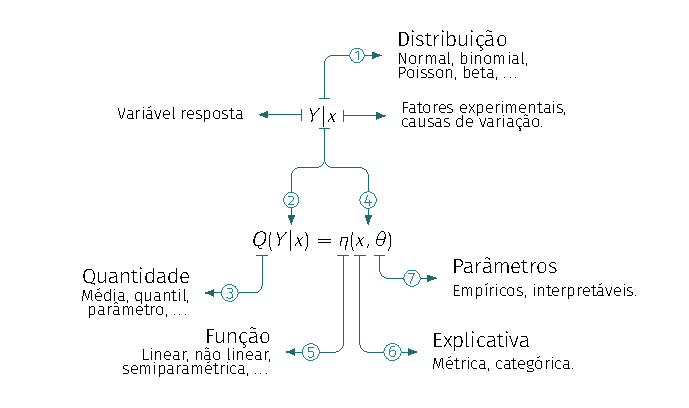
\includegraphics[width=11cm]{./img/modelos_regressao} \end{center}
\end{frame}

\begin{frame}{Modelos de regressão}
\protect\hypertarget{modelos-de-regressuxe3o-5}{}
\beginAHalfColumnT

\begin{enumerate}
\tightlist
\item
  \textbf{Definição do problema.}

  \begin{itemize}
  \tightlist
  \item
    Qual o fenômeno aleatório de interesse?
  \item
    Que fatores externos podem afetar este fenômeno?
  \end{itemize}
\item
  \textbf{Planejamento do estudo e coleta de dados.}

  \begin{itemize}
  \tightlist
  \item
    Estudo observacional x estudo experimental.
  \item
    Representação tabular.
  \end{itemize}
\end{enumerate}

\endColumns
\beginAHalfColumnT

\begin{enumerate}
\setcounter{enumi}{2}
\tightlist
\item
  \textbf{Análise dos dados via regressão.}

  \begin{itemize}
  \tightlist
  \item
    Distribuição de probabilidade.
  \item
    Especificação do modelo.
  \item
    Obtenção dos parâmetros (ajuste).
  \item
    Diagnóstico.
  \end{itemize}
\item
  \textbf{Interpretação dos resultados.}

  \begin{itemize}
  \tightlist
  \item
    Quais os fatores externos apresentam ou não impacto sobre o
    fenômeno.
  \item
    Qual a dimensão desse impacto.
  \end{itemize}
\end{enumerate}

\endColumns
\end{frame}

\begin{frame}{Modelos de regressão}
\protect\hypertarget{modelos-de-regressuxe3o-6}{}
\begin{itemize}
    \itemsep 2ex

  \item Existem modelos univariados e multivariados. 
  
    \begin{itemize}
      \item \textbf{Univariados}: apenas uma variável resposta.
      \item \textbf{Multivariados}: mais de uma variável resposta.
    \end{itemize}

  \item Em ambos os casos o interesse é avaliar o \textbf{efeito de variáveis explicativas}.
  
  \item Existem inúmeras classes de modelos de regressão, dentre elas: 
  \begin{itemize}
  \item Modelo linear normal.
  \item Modelos lineares generalizados.
  \item \textbf{Modelos multivariados de covariância linear generalizada.}
\end{itemize}

  \end{itemize}
\end{frame}

\begin{frame}{Modelo linear normal}
\protect\hypertarget{modelo-linear-normal}{}
\begin{itemize}
    \itemsep 2ex

  \item O modelo linear normal \citep{galton} ficou famoso por suas \textbf{facilidades computacionais}. 
  
  \item Possui \textbf{pressupostos} difíceis de serem atendidos na prática.
    \begin{itemize}
      \item Independência.
      \item Normalidade.
      \item Variância constante.
    \end{itemize}
  
  \item Diversas técnicas foram propostas para solucionar casos em que os pressupostos fossem violados.
  
  \end{itemize}
\end{frame}

\begin{frame}{Modelos lineares generalizados}
\protect\hypertarget{modelos-lineares-generalizados}{}
\begin{itemize}
    \itemsep 2ex

  \item O \textbf{avanço computacional} permitiu o surgimento de modelos mais gerais que necessitavam de \textbf{processos iterativos} para estimação dos parâmetros. 
  
  \item Surgem os modelos lineares generalizados (\textbf{GLMs}) \citep{Nelder72}. 
  
  \item Os GLMs permitem utilizar qualquer membro da \textbf{família exponencial de distribuições}.

  \item Casos especiais: Bernoulli, binomial, Poisson, normal, gama, normal inversa, entre outras.
  
  \end{itemize}
\end{frame}

\begin{frame}{Modelos multivariados de covariância linear generalizada}
\protect\hypertarget{modelos-multivariados-de-covariuxe2ncia-linear-generalizada}{}
\begin{itemize}
    \itemsep 2ex
  
  \item Apesar do grande potencial, os GLMs apresentam três importantes \textbf{restrições}:
    \begin{enumerate}
      \itemsep 2ex
    
      \item A incapacidade de lidar com \textbf{observações dependentes}. 
      \item A incapacidade de lidar com \textbf{múltiplas respostas} simultaneamente.
      \item Leque reduzido de \textbf{distribuições disponíveis}. 
    \end{enumerate}

  \item Os modelos multivariados de covariância linear generalizada (\textbf{McGLMs}) \citep{Bonat16} contornam estas restrições.

  \end{itemize}
\end{frame}

\begin{frame}{Modelos multivariados de covariância linear generalizada}
\protect\hypertarget{modelos-multivariados-de-covariuxe2ncia-linear-generalizada-1}{}
\begin{itemize}
   
   \itemsep 2ex
   
  \item Configuram uma estrutura geral para análise via modelos de regressão.
  
  \item Comporta \textbf{múltiplas respostas} de diferentes naturezas.
  
  \item Pode-se ajustar modelos com \textbf{diferentes preditores e distribuições} para cada resposta.
  
  \item Os modelos levam em conta a \textbf{correlação entre observações} do conjunto de dados. 

\end{itemize}
\end{frame}

\begin{frame}{Modelos multivariados de covariância linear generalizada}
\protect\hypertarget{modelos-multivariados-de-covariuxe2ncia-linear-generalizada-2}{}
\begin{itemize}
   
   \itemsep 2ex
  
  \item Os parâmetros são interpretáveis:
  
    \begin{itemize}
    
    \itemsep 2ex
      
      \item \textbf{Parâmetros de regressão}: efeito das variáveis explicativas sobre as respostas.
      
      \item \textbf{Parâmetros de dispersão}: impacto da correlação entre unidades.
      
      \item \textbf{Parâmetros de potência}: indicativo de qual distribuição se adequa ao problema.
      
      \item \textbf{Parâmetros correlação}: força de associação entre respostas.
      
    \end{itemize}

  \item As estimativas dos parâmetros podem ser estudadas por meio de \textbf{testes de hipóteses}.
\end{itemize}
\end{frame}

\begin{frame}{Testes de hipóteses em modelos de regressão}
\protect\hypertarget{testes-de-hipuxf3teses-em-modelos-de-regressuxe3o}{}
\begin{itemize}
    \itemsep 2ex
  
  \item Usados para verificar se a \textbf{retirada de determinada variável} explicativa do modelo geraria uma \textbf{perda no ajuste}.
  
  \item Os três testes mais usados são:

    \begin{itemize}
      \item O teste da razão de verossimilhanças \citep{trv}.
      \item O teste do multiplicador de lagrange ou teste escore \citep{score1,score2,score3}.
      \item \textbf{O teste Wald \citep{wald}.}
    \end{itemize}
  
  \item São baseados na função de verossimilhança dos modelos.
  
  \item São \textbf{assintóticamente equivalentes} \citep{engle}.
  
  \end{itemize}
\end{frame}

\begin{frame}{Testes de hipóteses em modelos de regressão}
\protect\hypertarget{testes-de-hipuxf3teses-em-modelos-de-regressuxe3o-1}{}
\textbf{Teste Wald}

\begin{itemize}

  \itemsep 2ex
  
  \item Requer apenas um modelo ajustado. 

  \item Consiste em verificar se existe evidência para afirmar que um ou mais parâmetros são iguais a valores postulados. 

  \item Avalia quão longe o valor estimado está do valor postulado. 

  \item É possível formular hipóteses para múltiplos parâmetros.

\end{itemize}
\end{frame}

\begin{frame}{ANOVA, MANOVA e testes de comparações múltiplas}
\protect\hypertarget{anova-manova-e-testes-de-comparauxe7uxf5es-muxfaltiplas}{}
Existe uma série de
\textbf{procedimentos baseados em testes de hipóteses}, tais como:

\begin{itemize}

  \itemsep 2ex
  
  \item Análise de variância (\textbf{ANOVA}).
  \item Análise de variância multivariada (\textbf{MANOVA}).
  \item Testes de \textbf{comparações múltiplas}.

\end{itemize}
\end{frame}

\begin{frame}{Temas abordados até aqui}
\protect\hypertarget{temas-abordados-atuxe9-aqui}{}
\begin{itemize}
  \itemsep 2ex
    
  \item Ciência de dados.

  \item Modelos de regressão.

  \item Classes de modelos de regressão (ênfase nos \textbf{McGLMs}).

  \item Testes de hipóteses em modelos de regressão (ênfase no \textbf{teste Wald}).

  \item Procedimentos baseados em testes de hipóteses (ênfase na \textbf{ANOVA, MANOVA e testes de comparações múltiplas}).

\end{itemize}
\end{frame}

\begin{frame}{Desafio e hipótese}
\protect\hypertarget{desafio-e-hipuxf3tese}{}
\begin{itemize}
  \itemsep 2ex
    
  \item Não há discussão a respeito da \textbf{construção de testes de hipóteses para os McGLMs.}    

  \item Contudo, os McGLMs apresentam os elementos necessários para utilizar o \textbf{teste Wald}:
    \begin{enumerate}
      \item Um vetor de estimativas dos parâmetros
      \item Uma matriz de variância e covariância destas estimativas.
    \end{enumerate}
    
  \item Das três opções clássicas de testes de hipóteses, o teste Wald se torna o mais atrativo para os McGLMs. 

\end{itemize}
\end{frame}

\begin{frame}{Objetivo}
\protect\hypertarget{objetivo}{}
\begin{enumerate}
  \itemsep 2ex
  
 \item Propor a utilização do \textbf{teste Wald} para realização de testes de hipóteses gerais sobre parâmetros de \textbf{regressão} e \textbf{dispersão} de \textbf{McGLMs}.

 \item Avaliar as propriedades e comportamento dos testes propostos com base em \textbf{estudos de simulação}.
 
 \item \textbf{Implementar} funções em R para testes de hipóteses, ANOVA, MANOVA e testes de comparações múltiplas para os McGLMs. 
 
 \item Motivar o potencial de aplicação das metodologias discutidas com base na \textbf{aplicação a conjuntos de dados reais}.

\end{enumerate}
\end{frame}

\begin{frame}{Contribuição}
\protect\hypertarget{contribuiuxe7uxe3o}{}
\begin{itemize}
  \itemsep 2ex
  
  \item Formas de \textbf{avaliar os parâmetros} estimados pelos McGLMs.

  \item Fornecer ferramentas para uma melhor \textbf{interpretação dos parâmetros} estimados, permitindo responder questões comuns no contexto de modelagem.
  
  \item \textbf{Extrair mais informações e conclusões} a respeito dos problemas modelados por meio dos McGLMs.

\end{itemize}
\end{frame}

\hypertarget{referencial-teuxf3rico}{%
\section{Referencial teórico}\label{referencial-teuxf3rico}}

\begin{frame}{Referencial teórico}
\end{frame}

\begin{frame}{Referencial teórico}
\protect\hypertarget{referencial-teuxf3rico-1}{}
\begin{enumerate}
    \itemsep 2ex
    
  \item McGLMs
    \begin{itemize}
      \item Elementos.
      \item Preditores lineares e matriciais.
      \item Funções de variância.
      \item Parâmetros.
      \item Estimação.
    \end{itemize}
    
  \item Testes de hipóteses
    \begin{itemize}
      \item Elementos de um teste de hipóteses.
      \item Testes de hipóteses em modelos de regressão.
      \item Teste Wald
      \item ANOVA e MANOVA.
      \item Testes de comparações múltiplas.
    \end{itemize}
\end{enumerate}
\end{frame}

\hypertarget{modelos-multivariados-de-covariuxe2ncia-linear-generalizada-3}{%
\section{Modelos multivariados de covariância linear
generalizada}\label{modelos-multivariados-de-covariuxe2ncia-linear-generalizada-3}}

\begin{frame}{Modelos multivariados de covariância linear generalizada}
\end{frame}

\begin{frame}{Modelos multivariados de covariância linear generalizada}
\protect\hypertarget{modelos-multivariados-de-covariuxe2ncia-linear-generalizada-4}{}
Para definição de um McGLM considere:

\begin{itemize}
  
  \itemsep 2ex
  
  \item $\boldsymbol{Y}_{N \times R} = \left \{ \boldsymbol{Y}_1, \dots, \boldsymbol{Y}_R \right \}$ uma matriz de \textbf{variáveis resposta}.
  
  \item $\boldsymbol{M}_{N \times R} = \left \{ \boldsymbol{\mu}_1, \dots, \boldsymbol{\mu}_R \right \}$ uma matriz de \textbf{valores esperados}.
  
  \item $\boldsymbol{X}_r$ denota uma \textbf{matriz de delineamento} $N \times k_r$.
  
  \item $\boldsymbol{\beta}_r$ denota um vetor $k_r \times 1$ de \textbf{parâmetros de regressão}.
  
\end{itemize}
\end{frame}

\begin{frame}{Modelos multivariados de covariância linear generalizada}
\protect\hypertarget{modelos-multivariados-de-covariuxe2ncia-linear-generalizada-5}{}
Considere ainda:

\begin{itemize}
  
  \itemsep 2ex
  
  \item $\Sigma_b$ uma \textbf{matriz de correlação} entre variáveis resposta, de ordem $R \times R$.
    
  \item $\Sigma_r$, $r = 1,..., R$, a \textbf{matriz de variância e covariância} para cada resposta $r$, de dimensão $NxN$:
  
$$
\Sigma_r = \mathrm{V}_r\left(\boldsymbol{\mu}_r; p_r\right)^{1/2}(\boldsymbol{\Omega}\left(\boldsymbol{\tau}_r\right))\mathrm{V}_r\left(\boldsymbol{\mu}_r; p_r\right)^{1/2}.
$$

Em que:

  \begin{itemize}
    \item $\mathrm{V}_r\left(\boldsymbol{\mu}; p\right)$ é uma matriz diagonal em que as entradas principais são dadas pela função de variância aplicada ao vetor $\boldsymbol{\mu}$. 
  
  \item $p_r$ é o parâmetro de potência. 
  
  \item $\boldsymbol{\Omega}\left(\boldsymbol{\tau}_r\right)$ a matriz de dispersão que descreve a parte da covariância dentro de cada variável resposta. 
  \end{itemize}
  
\end{itemize}
\end{frame}

\begin{frame}{Preditor linear matricial}
\protect\hypertarget{preditor-linear-matricial}{}
\begin{itemize}
  
  \itemsep 2ex
  
  \item A matriz $\boldsymbol{\Omega}(\boldsymbol{\tau}_r)$ descreve a estrutura de \textbf{correlação entre as observações} da amostra.
  
  \item É modelada através de um \textbf{preditor linear matricial} combinado com uma função de ligação de covariância:

$$
h\left \{ \boldsymbol{\Omega}(\boldsymbol{\tau}_r) \right \} = \tau_{r0}Z_0 + \ldots + \tau_{rD}Z_D
$$
  
  \begin{itemize}
  
  \itemsep 2ex
  
  \item $h()$ é a função de ligação de covariância.
  
  \item $Z_{rd}$ com $d$ = 0,$\ldots$, D são matrizes que representam a estrutura de covariância presente em cada variável resposta $r$.
  
  \item $\boldsymbol{\tau_r}$ = $(\tau_{r0}, \ldots, \tau_{rD})$ é um vetor $(D + 1) \times 1$ de parâmetros de dispersão. 
  
\end{itemize}

\end{itemize}
\end{frame}

\begin{frame}{Funções de variância}
\protect\hypertarget{funuxe7uxf5es-de-variuxe2ncia}{}
\begin{enumerate}
  \item \textbf{Função de variância potência} \citep{Jorgensen87, Jorgensen97}.
  
    \begin{itemize}
      \item Família \textbf{Tweedie} de distribuições.
      \item $\vartheta\left(\boldsymbol{\mu}; p\right) = \mu^p$.
      \item Casos particulares: normal ($p$ = 0), Poisson ($p$ = 1), gama ($p$ = 2) e normal inversa ($p$ = 3).
    \end{itemize}

  
  \item \textbf{Função de dispersão Poisson–Tweedie} \citep{Jorgensen15}.
  
    \begin{itemize}
      \item Família \textbf{Poisson-Tweedie} de distribuições.
      \item $\vartheta\left(\boldsymbol{\mu}; p\right) = \mu + \mu^p$.
      \item Casos particulares: Hermite ($p$ = 0), Neyman tipo A ($p$ = 1), binomial negativa ($p$ = 2) e Poisson–inversa gaussiana (p = $3$).
      
    \end{itemize}

  \item \textbf{Função de variância binomial.} 
  
    \begin{itemize}
      \item $\vartheta(\boldsymbol{\mu}) = \mu(1 - \mu)$.
      \item Acomoda \textbf{respostas binárias} ou \textbf{restritas a um intervalo}.
    \end{itemize}

\end{enumerate}
\end{frame}

\begin{frame}{Modelos multivariados de covariância linear
generalizada\}}
\protect\hypertarget{modelos-multivariados-de-covariuxe2ncia-linear-generalizada-6}{}
Os McGLMs são definidos por:

\begin{center}
$\mathrm{E}(\boldsymbol{Y}) = \boldsymbol{M} = \{g_1^{-1}(\boldsymbol{X}_1 \boldsymbol{\beta}_1), \ldots, g_R^{-1}(\boldsymbol{X}_R \boldsymbol{\beta}_R)\}$

$\mathrm{Var}(\boldsymbol{Y}) = \boldsymbol{C} = \boldsymbol{\Sigma}_R \overset{G} \otimes \boldsymbol{\Sigma}_b$

\end{center}

Em que:

\begin{itemize}
  
  \item $\boldsymbol{\Sigma}_R \overset{G} \otimes \boldsymbol{\Sigma}_b = \mathrm{Bdiag}(\tilde{\boldsymbol{\Sigma}}_1, \ldots, \tilde{\boldsymbol{\Sigma}}_R) (\boldsymbol{\Sigma}_b \otimes \boldsymbol{I}) \mathrm{Bdiag}(\tilde{\boldsymbol{\Sigma}}_1^\top, \ldots, \tilde{\boldsymbol{\Sigma}}_R^\top)$ é o produto generalizado de Kronecker.
  
  \item $\tilde{\boldsymbol{\Sigma}}_r$ denota a matriz triangular inferior da decomposição de Cholesky da matriz ${\boldsymbol{\Sigma}}_r$.
  
  \item $\mathrm{Bdiag()}$ denota a matriz bloco-diagonal.
  
  \item $\boldsymbol{I}$ uma matriz identidade $N \times N$.
  
  \item $g_r()$ são as tradicionais funções de ligação.
  
\end{itemize}
\end{frame}

\begin{frame}{Modelos multivariados de covariância linear generalizada}
\protect\hypertarget{modelos-multivariados-de-covariuxe2ncia-linear-generalizada-7}{}
\begin{itemize}

\itemsep 2ex
  
  \item Parâmetros estimados nos McGLMs:
    \begin{enumerate}
      \item \textbf{Regressão.}
      \item \textbf{Dispersão.}
      \item \textbf{Potência.}
      \item \textbf{Correlação.}
    \end{enumerate}
  
  \item Todas estas quantidades são \textbf{interpretáveis} e são estimadas com base nos dados.
  
  \item A estimação é feita por meio de \textbf{funções de estimação}.
    \begin{enumerate}
      \item \textbf{Função quasi-score} para parâmetros de regressão. 
      \item \textbf{Função de estimação de Pearson} para os demais parâmetros. 
    \end{enumerate}

\end{itemize}
\end{frame}

\begin{frame}{Funções de estimação}
\protect\hypertarget{funuxe7uxf5es-de-estimauxe7uxe3o}{}
\begin{center}
$\psi_{\boldsymbol{\beta}}(\boldsymbol{\beta}, \boldsymbol{\lambda}) = \boldsymbol{D}^\top \boldsymbol{C}^{-1}(\mathcal{Y} - \mathcal{M})$

$\psi_{\boldsymbol{\lambda}_i}(\boldsymbol{\beta}, \boldsymbol{\lambda}) = \mathrm{tr}(W_{\boldsymbol{\lambda}i} (\boldsymbol{r}^\top\boldsymbol{r} - \boldsymbol{C})),  i = 1,.., Q$
\end{center}

Em que:

\begin{itemize}
  
  \item \normalsize $\boldsymbol{\beta}_r$ denota um vetor $k_r \times 1$ de parâmetros de regressão.
  
  \item \normalsize $\boldsymbol{\lambda}$ é um vetor $Q \times 1$ de parâmetros de dispersão.
  
  \item \normalsize $\mathcal{Y}$ é um vetor $NR \times 1$ com os valores da matriz de variáveis respostas $Y_{N \times R}$ empilhados.
  
  \item \normalsize $\mathcal{M}$ é um vetor $NR \times 1$ com os valores da matriz de valores esperados $M_{N \times R}$ empilhados.
  
  \item \normalsize $\boldsymbol{D} = \nabla_{\boldsymbol{\beta}} \mathcal{M}$ 
é uma matriz $NR \times K$, e $\nabla_{\boldsymbol{\beta}}$ denota o 
operador gradiente.
  
  \item \normalsize $W_{\boldsymbol{\lambda}i} = -\frac{\partial
    \boldsymbol{C}^{-1}}{\partial \boldsymbol{\lambda}_i}$ 
    
  \item \normalsize $\boldsymbol{r} = (\mathcal{Y} - \mathcal{M})$
  
\end{itemize}
\end{frame}

\begin{frame}{Distribuição assintótica e algoritmo de estimação}
\protect\hypertarget{distribuiuxe7uxe3o-assintuxf3tica-e-algoritmo-de-estimauxe7uxe3o}{}
\begin{itemize}

  \item Para resolver o sistema de equações $\psi_{\boldsymbol{\beta}} = 0$ e $\psi_{\boldsymbol{\lambda}} = 0$ faz-se uso do algoritmo \textbf{Chaser modificado}:

$$
\begin{matrix}
\boldsymbol{\beta}^{(i+1)} = \boldsymbol{\beta}^{(i)}- S_{\boldsymbol{\beta}}^{-1} \psi \boldsymbol{\beta} (\boldsymbol{\beta}^{(i)}, \boldsymbol{\lambda}^{(i)}), \\ 
\boldsymbol{\lambda}^{(i+1)} = \boldsymbol{\lambda}^{(i)}\alpha S_{\boldsymbol{\lambda}}^{-1} \psi \boldsymbol{\lambda} (\boldsymbol{\beta}^{(i+1)}, \boldsymbol{\lambda}^{(i)}).
\end{matrix}
$$

  \item Seja $\boldsymbol{\hat{\theta}} = (\boldsymbol{\hat{\beta}^{\top}}, \boldsymbol{\hat{\lambda}^{\top}})^{\top}$ o estimador baseado em funções de estimação de $\boldsymbol{\theta}$.
  
  \item A \textbf{distribuição assintótica} de $\boldsymbol{\hat{\theta}}$ é:

$$
\boldsymbol{\hat{\theta}} \sim N(\boldsymbol{\theta}, J_{\boldsymbol{\theta}}^{-1}),
$$

\noindent $J_{\boldsymbol{\theta}}^{-1}$ é a inversa da matriz de informação de Godambe, dada por
  
$$J_{\boldsymbol{\theta}}^{-1} = S_{\boldsymbol{\theta}}^{-1} V_{\boldsymbol{\theta}} S_{\boldsymbol{\theta}}^{-\top},$$ 

\noindent em que $S_{\boldsymbol{\theta}}^{-\top} = (S_{\boldsymbol{\theta}}^{-1})^{\top}.$

\end{itemize}
\end{frame}

\hypertarget{testes-de-hipuxf3teses}{%
\section{Testes de hipóteses}\label{testes-de-hipuxf3teses}}

\begin{frame}{Testes de hipóteses}
\end{frame}

\begin{frame}{Testes de hipóteses}
\protect\hypertarget{testes-de-hipuxf3teses-1}{}
\begin{itemize}
    \itemsep 2ex
  
  \item Inferência: \textbf{inferir} conclusões válidas a respeito de uma \textbf{população} por meio do estudo de uma \textbf{amostra}.
  
  \item Problemas de inferência estatística são:
    \begin{enumerate}
    
      \itemsep 2ex
      
      \item \textbf{Estimação} de parâmetros com base em informação amostral.
      
      \item \textbf{Testes de hipóteses}.
        \begin{itemize}
          \item Com base na evidência amostral, podemos considerar que dado parâmetro tem determinado valor?
        \end{itemize}
    
    \end{enumerate}
  
  \end{itemize}
\end{frame}

\begin{frame}{Testes de hipóteses}
\protect\hypertarget{testes-de-hipuxf3teses-2}{}
\begin{itemize}
    \itemsep 2ex
  
  \item São postuladas 2 hipóteses, chamadas de \textbf{nula} e \textbf{alternativa}.
  
  \item Avalia-se uma \textbf{estatística de teste}.
  
  \item Com base no valor da estatística e de acordo com sua distribuição de probabilidade, toma-se a decisão de \textbf{rejeitar} ou \textbf{não rejeitar} a hipótese nula.
    
  \item Seja $\pi$ um parâmetro, um teste de hipóteses sobre $\pi$ é dado por:
  
$$
\left\{\begin{matrix}
H_0: \pi = \pi_0 \\ 
H_1: \pi \neq \pi_0
\end{matrix}\right.
$$  
  
  \end{itemize}
\end{frame}

\begin{frame}{Testes de hipóteses}
\protect\hypertarget{testes-de-hipuxf3teses-3}{}
Desfechos possíveis:

\begin{table}[]
\begin{tabular}{l|cc}
\hline
\multicolumn{1}{c|}{}    & \textbf{Rejeita $H_0$} & \textbf{Não Rejeita $H_0$} \\ \hline
\textbf{$H_0$ verdadeira} & Erro tipo I           & Decisão correta           \\
\textbf{$H_0$ falsa}      & Decisão correta       & Erro tipo II              \\ \hline
\end{tabular}
\label{tab:my-table}
\end{table}

\begin{itemize}
    \itemsep 2ex
  
  \item A probabilidade do erro do tipo I recebe o nome de \textbf{nível de significância}.
  
  \item A probabilidade de se rejeitar corretamente $H_0$ recebe o nome de \textbf{poder do teste}.
  
  \item A probabilidade de a estatística de teste tomar um valor igual ou mais extremo do que aquele que foi observado recebe o nome de \textbf{valor-p}.
    
  \end{itemize}
\end{frame}

\begin{frame}{Testes de hipóteses em modelos de regressão}
\protect\hypertarget{testes-de-hipuxf3teses-em-modelos-de-regressuxe3o-2}{}
\begin{itemize}
  \itemsep 2ex

  \item \textbf{Testes de hipóteses são ferramentas gerais} que podem ser aplicadas em problemas de regressão.
  
  \item Modelos de regressão: modelar uma ou mais variáveis em função de um conjunto de variáveis explicativas. 

  \item Modelos contêm parâmetros que são quantidades desconhecidas que estabelecem a relação entre as variáveis sob o modelo. 

  \item Para avaliar os parâmetros de um modelo testes de hipóteses são usados.

\end{itemize}
\end{frame}

\begin{frame}{Teste Wald em modelos de regressão}
\protect\hypertarget{teste-wald-em-modelos-de-regressuxe3o}{}
\begin{itemize}
  \itemsep 2ex

  \item Consiste em verificar se existe evidência suficiente nos dados para afirmar que um ou mais parâmetros são iguais a valores especificados.
  
  \item Avalia a distância entre as estimativas dos parâmetros e um conjunto de valores postulados.
  
  \item Esta diferença é ainda padronizada por medidas de precisão das estimativas dos parâmetros. 

  \item Quanto maior for esta distância padronizada, menores são as evidências a favor da hipótese de que os valores estimados são iguais aos valores postulados.


  \end{itemize}
\end{frame}

\begin{frame}{Teste Wald em modelos de regressão}
\protect\hypertarget{teste-wald-em-modelos-de-regressuxe3o-1}{}
Considere um problema de regressão em que:

\begin{itemize}

  \itemsep 2ex
  
  \item $\boldsymbol{\beta}$ um vetor $k\times1$ \textbf{parâmetros de regressão}.
    
  \item $\boldsymbol{\hat\beta}$ as \textbf{estimativas} dos parâmetros.
    
  \item $\boldsymbol{L}$ uma \textbf{matriz de especificação das hipóteses}, de dimensão $s \times k$.  
  
  \item $\boldsymbol{c}$ um vetor de \textbf{valores postulados} de dimensão $s$.
    
  \end{itemize}
\end{frame}

\begin{frame}{Teste Wald em modelos de regressão}
\protect\hypertarget{teste-wald-em-modelos-de-regressuxe3o-2}{}
\begin{itemize}

  \itemsep 2ex
  
  \item As hipóteses podem ser descritas como:

$$
\left\{\begin{matrix}
H_0: \boldsymbol{L}\boldsymbol{\beta} = \boldsymbol{c} \\ 
H_1: \boldsymbol{L}\boldsymbol{\beta} \neq \boldsymbol{c}
\end{matrix}\right.
$$

  \item A estatística de teste é dada por:

$$
WT = (\boldsymbol{L\hat\beta} - \boldsymbol{c})^T \ (\boldsymbol{L \ Var^{-1}(\hat\beta) \ L^T})^{-1} \ (\boldsymbol{L\hat\beta} - \boldsymbol{c}).
$$

 \item  WT $\sim \chi^2_s$.

\end{itemize}
\end{frame}

\begin{frame}{ANOVA e MANOVA}
\protect\hypertarget{anova-e-manova}{}
\begin{itemize}

  \itemsep 2ex

  \item \textbf{Testes sucessivos impondo restrições} ao modelo original. 

  \item Avaliar o efeito das variáveis explicativas. 
  
  \item Caso univariado: \textbf{ANOVA}. Caso multivariado: \textbf{MANOVA}.

  \item O quadro de ANOVA ou MANOVA contém em cada linha: 
    \begin{enumerate}
      \item A variável. 
      \item O valor da estatística de teste. 
      \item Os graus de liberdade. 
      \item Um valor-p.
    \end{enumerate}

  \item É possível gerar quadros de análise de variância por meio do teste Wald.

  \end{itemize}
\end{frame}

\begin{frame}{Testes de comparações múltiplas}
\protect\hypertarget{testes-de-comparauxe7uxf5es-muxfaltiplas}{}
\begin{itemize}

  \itemsep 2ex

  \item Usado quando a ANOVA aponta para \textbf{efeito significativo de uma variável categórica}.

  \item \textbf{Comparações aos pares} a fim de detectar para quais níveis da variável categórica os valores da resposta se alteram.

  \item Pode ser avaliada utilizando o teste Wald. 

  \item Por meio da correta especificação da matriz $\boldsymbol{L}$, é possível \textbf{avaliar hipóteses sobre qualquer possível contraste} entre os níveis de uma determinada variável categórica. 

\end{itemize}
\end{frame}

\hypertarget{trabalhos-relacionados}{%
\section{Trabalhos relacionados}\label{trabalhos-relacionados}}

\begin{frame}{Trabalhos relacionados}
\end{frame}

\begin{frame}{Trabalhos relacionados}
\protect\hypertarget{trabalhos-relacionados-1}{}
\begin{itemize}
  \itemsep 2ex
  
  \item Propostas que visam \textbf{contornar restrições dos GLMs} e como são efetuados testes de hipóteses para estas propostas.
  
  \item Propostas univariadas e multivariadas.
  
  \item Efeitos aleatórios.
  
  \item Correção de erros padrões.
  
  \item Grande variedade de modelos de regressão multivariados para fins específicos.
  
\end{itemize}
\end{frame}

\begin{frame}{Trabalhos relacionados}
\protect\hypertarget{trabalhos-relacionados-2}{}
\begin{itemize}
  \itemsep 2ex
  
  \item Efeitos aleatórios para acomodar correlação entre observações.
    \begin{itemize}
      \item Modelos lineares generalizados mistos (\textbf{GLMM}).
      \item Modelos lineares generalizados multivariados mistos (\textbf{MGLMM}).
    \end{itemize}

  \item Equações de estimação generalizadas (\textbf{GEE}).

  \item Modelos aditivos generalizados para locação, escala e forma (\textbf{GAMLSS}).
  
\end{itemize}
\end{frame}

\begin{frame}{Trabalhos relacionados}
\protect\hypertarget{trabalhos-relacionados-3}{}
Grande variedade de modelos de regressão multivariados para fins
específicos.

\begin{itemize}
  
  \item Análise de contagens multivariadas em que os testes usuais se aplicam \citep{zhang2017regression}.  

  \item Modelo de regressão multivariado com distribuição Poisson inversa gaussiana em que testes de hipóteses ao estilo da razão de verossimilhanças se aplicam \citep{mardalena2020parameter}. 

  \item Modelo de regressão Poisson zero inflacionado multivariado em que o teste da razão de verossimilhanças e o teste Wald se aplicam \citep{sari2021estimation}.
  
  \item Modelo de regressão multivariado gamma em que um análogo do teste da razão de verossimilhanças e o teste Wald se aplicam \citep{rahayu2020multivariate}.

  \item Dentre outros.
  
\end{itemize}
\end{frame}

\hypertarget{teste-wald-para-mcglms}{%
\section{Teste Wald para McGLMs}\label{teste-wald-para-mcglms}}

\begin{frame}{Teste Wald para McGLMs}
\end{frame}

\begin{frame}{Teste Wald para McGLMs}
\protect\hypertarget{teste-wald-para-mcglms-1}{}
\begin{enumerate}
  \itemsep 2ex
    
  \item Definição das hipóteses.
  \item Estatística de teste.
  \item Distribuição.
  \item Hipóteses comuns.
  \item Construção da matriz $\boldsymbol{L}$.
  \item Exemplos.
  
\end{enumerate}
\end{frame}

\begin{frame}{Hipóteses}
\protect\hypertarget{hipuxf3teses}{}
\[H_0: \boldsymbol{L}\boldsymbol{\theta^{*}} = \boldsymbol{c} \ vs \ H_1: \boldsymbol{L}\boldsymbol{\theta^{*}} \neq \boldsymbol{c}.\]

Em que:

\begin{itemize}
  
  \item $\boldsymbol{\theta^{*}}$ é o vetor de dimensão $h \times 1$ de parâmetros de regressão, dispersão e potência do modelo. 
  
  \item Em que $\boldsymbol{L}$ é a matriz de especificação das hipóteses a serem testadas, tem dimensão $s \times h$. 
  
  \item $\boldsymbol{c}$ é um vetor de dimensão $s \times 1$ com os valores sob hipótese nula.

\end{itemize}
\end{frame}

\begin{frame}{Estatística de teste}
\protect\hypertarget{estatuxedstica-de-teste}{}
\[W = (\boldsymbol{L\hat\theta^{*}} - \boldsymbol{c})^T \ (\boldsymbol{L \ J^{\boldsymbol{*}-1} \ L^T})^{-1} \ (\boldsymbol{L\hat\theta^{*}} - \boldsymbol{c}).\]

Em que:

\begin{itemize}
  \item $\boldsymbol{L}$ é a matriz da especificação das hipóteses, tem dimensão $s \times h$. 

  \item $\boldsymbol{\hat\theta^{*}}$ é o vetor de dimensão $h \times 1$ com todas as estimativas dos parâmetros de regressão, dispersão e potência. 

  \item $\boldsymbol{c}$ é um vetor de dimensão $s \times 1$ com os valores sob hipótese nula. 

  \item E $\boldsymbol{J^{\boldsymbol{*}-1}}$ é a inversa da matriz de informação de Godambe desconsiderando os parâmetros de correlação, de dimensão $h \times h$. 
  
  \item $W \sim \chi^2_s$

\end{itemize}
\end{frame}

\begin{frame}{Hipóteses comuns}
\protect\hypertarget{hipuxf3teses-comuns}{}
\begin{itemize}
  \itemsep 2ex
  
  \item Costuma ser de interesse formular hipóteses:
    \begin{enumerate}
      \itemsep 1ex
      \item Para \textbf{parâmetros individuais}.
      \item Para \textbf{múltiplos parâmetros}.
      \item Para avaliar \textbf{igualdade de parâmetros}.
      \item Sobre parâmetros de regressão ou dispersão para \textbf{respostas sob mesmo preditor}.
      \item Sobre \textbf{contrastes}.
\end{enumerate}
  
  \item O elemento chave é a correta especificação da matriz $\boldsymbol{L}$.
  
\end{itemize}
\end{frame}

\begin{frame}{Construção da matriz \(\boldsymbol{L}\)}
\protect\hypertarget{construuxe7uxe3o-da-matriz-boldsymboll}{}
\begin{itemize}
  \itemsep 2ex
  
  \item Cada coluna da matriz $\boldsymbol{L}$ corresponde a um dos $h$ parâmetros de $\boldsymbol{\theta^{*}}$. 
  
  \item Cada linha corresponde a uma restrição. 

  \item A matriz é composta por valores iguais a 0, 1 e eventualmente -1.
  
  \item O produto $\boldsymbol{L}\boldsymbol{\theta^{*}}$ deve resultar nas hipóteses de interesse.

\end{itemize}
\end{frame}

\begin{frame}{Exemplo}
\protect\hypertarget{exemplo}{}
\textbf{Considere o problema:}

\begin{itemize}
  
  \item Investigar se uma variável numérica $X_1$ possui efeito sobre $Y_1$ e $Y_2$. 
  
  \item Amostra com $N$ observações, para cada observação obteve-se $X_1$, $Y_1$ e $Y_2$.

  \item Um McGLM bivariado, pode ter preditor dado por

\end{itemize}

\[
g_r(\mu_r) = \beta_{r0} + \beta_{r1} X_1
\]

\beginAHalfColumnT
  \begin{itemize}
    \itemsep 1ex
    \item $r$ denota a variável resposta, r = 1,2.
    \item $\beta_{r0}$ representa o intercepto.
    \item $\beta_{r1}$ um parâmetro de regressão associado a uma variável $X_1$. 
  \end{itemize}  
\endColumns
\beginAHalfColumnT

\begin{itemize}
    \itemsep 1ex
    \item Apenas um parâmetro de dispersão $\tau_{r0}$.
    \item Unidades independentes, logo $Z_0 = I$.
    \item Parâmetros de potência foram fixados.
  \end{itemize}

\endColumns
\end{frame}

\begin{frame}{Exemplo}
\protect\hypertarget{exemplo-1}{}
\[
g_r(\mu_r) = \beta_{r0} + \beta_{r1} X_1
\]

\beginAHalfColumnT

\textbf{Trata-se de um problema com:}

\begin{itemize}
  \itemsep 1ex
  \item Duas variáveis resposta.
  \item Apenas uma variável explicativa.
  \item Observações independentes.
\end{itemize}

\endColumns
\beginAHalfColumnT

\textbf{Podem ser perguntas de interesse:}

\begin{itemize}
  \itemsep 1ex
  \item Existe efeito da variável $X_1$ apenas sobre a primeira resposta?
  \item É possível que a variável $X_1$ possua efeito sobre as duas respostas ao mesmo tempo?
  \item É possível que o efeito da variável seja o mesmo para ambas as respostas? 
\end{itemize}

\endColumns
\end{frame}

\begin{frame}{Exemplo 1: hipótese para múltiplos parâmetros}
\protect\hypertarget{exemplo-1-hipuxf3tese-para-muxfaltiplos-paruxe2metros}{}
\begin{itemize}
  \itemsep 2ex
  
  \item Efeito da variável explicativa sobre ambas as respostas.
  
  \item Hipóteses: 
  
$$H_0: \beta_{r1} = 0 \ vs \ H_1: \beta_{r1} \neq 0$$  

  \item De forma equivalente

\end{itemize}

\[
H_0: 
\begin{pmatrix}
\beta_{11} \\ 
\beta_{21}
\end{pmatrix} 
= 
\begin{pmatrix}
0 \\ 
0
\end{pmatrix}
\ vs \ 
H_1: 
\begin{pmatrix}
\beta_{11} \\ 
\beta_{21}
\end{pmatrix} 
\neq
\begin{pmatrix}
0 \\ 
0 
\end{pmatrix}.
\]
\end{frame}

\begin{frame}{Exemplo 1: hipótese para múltiplos parâmetros}
\protect\hypertarget{exemplo-1-hipuxf3tese-para-muxfaltiplos-paruxe2metros-1}{}
Notação do teste Wald:

\[H_0: \boldsymbol{L}\boldsymbol{\theta^{*}} = \boldsymbol{c} \ vs \ H_1: \boldsymbol{L}\boldsymbol{\theta^{*}} \neq \boldsymbol{c}.\]

\begin{itemize}
  
    \item $\boldsymbol{\theta^{*T}}$ = $\begin{bmatrix} \beta_{10} \  \beta_{11} \ \beta_{20} \ \beta_{21} \ \tau_{11} \ \tau_{21} \end{bmatrix}$.

    \item $\boldsymbol{L} = \begin{bmatrix} 0 & 1 & 0 & 0 & 0 & 0 \\
0 & 0 & 0 & 1 & 0 & 0 \end{bmatrix}.$
 
  \item $\boldsymbol{c} = \begin{bmatrix} 0 \\ 0 \end{bmatrix}.$

  \end{itemize}
\end{frame}

\begin{frame}{Exemplo 2: hipótese de igualdade de parâmetros}
\protect\hypertarget{exemplo-2-hipuxf3tese-de-igualdade-de-paruxe2metros}{}
\begin{itemize}
  \itemsep 2ex
  
  \item Igualdade do efeito de $X_1$ para as respostas.

  \item Hipóteses:

$$
H_0: \beta_{11} - \beta_{21} = 0 \ vs \ H_1: \beta_{11} - \beta_{21} \neq 0,
$$

  \item Notação do teste Wald:
  
$$H_0: \boldsymbol{L}\boldsymbol{\theta^{*}} = \boldsymbol{c} \ vs \ H_1: \boldsymbol{L}\boldsymbol{\theta^{*}} \neq \boldsymbol{c}.$$  

  \begin{itemize}
  
    \item $\boldsymbol{\theta^{*T}}$ = $\begin{bmatrix} \beta_{10} \  \beta_{11} \ \beta_{20} \ \beta_{21} \ \tau_{11} \ \tau_{21} \end{bmatrix}$.

    \item $\boldsymbol{L} = \begin{bmatrix} 0 & 1 & 0 & -1 & 0 & 0  \end{bmatrix}.$
 
  \item $\boldsymbol{c}$ = $\begin{bmatrix} 0 \end{bmatrix}.$ 

  \end{itemize}
  
\end{itemize}
\end{frame}

\begin{frame}{ANOVA e MANOVA}
\protect\hypertarget{anova-e-manova-1}{}
\begin{itemize}
    \itemsep 2ex

  \item Com base na adaptação do teste Wald propostas, buscamos propor \textbf{ANOVAs e MANOVAs usando o teste Wald}.

  \item Propomos 3 tipos diferentes de análises de variância, nomeadas tipo I, II e III.

  \item Cada linha do quadro corresponde uma hipótese. Portanto, basta especificar uma matriz $\boldsymbol{L}$.

  \item As ANOVAs retornam \textbf{um quadro para cada resposta}.

  \item As MANOVAs retornam \textbf{um único quadro}. 
\end{itemize}
\end{frame}

\begin{frame}{Exemplo}
\protect\hypertarget{exemplo-2}{}
\textbf{Considere o problema:}

\begin{itemize}
  
  \item Investigar se duas variáveis numéricas ($X_1$ e $X_2$) possuem efeito sobre $Y_1$ e $Y_2$.
  
  \item Amostra com $N$ observações, para cada observação obteve-se $X_1$, $X_2$, $Y_1$ e $Y_2$.

  \item Um McGLM bivariado, pode ter preditor dado por

\end{itemize}

\[
g_r(\mu_r) = \beta_{r0} + \beta_{r1} X_1 + \beta_{r2} X_2 + \beta_{r3} X_1X_2.
\] \beginAHalfColumnT

\begin{itemize}
  \itemsep 1ex
  \item $r$ denota a variável resposta, r = 1,2.
  \item $\beta_{r0}$ representa o intercepto.
  \item $\beta_{r1}$ um parâmetro de regressão associado a uma variável $X_1$. 
  \item $\beta_{r2}$ um parâmetro de regressão associado a uma variável $X_2$.
\end{itemize}  
\endColumns    
\beginAHalfColumnT

\begin{itemize}
  \itemsep 1ex
  \item $\beta_{r3}$ um parâmetro de regressão associado a interação entre $X_1$ e $X_2$. 
  \item Apenas um parâmetro de dispersão $\tau_{r0}$.
  \item Unidades independentes, logo $Z_0 = I$.
  \item Parâmetros de potência foram fixados.
\end{itemize}

\endColumns
\end{frame}

\begin{frame}{ANOVA e MANOVA tipo II}
\protect\hypertarget{anova-e-manova-tipo-ii}{}
\[
g_r(\mu_r) = \beta_{r0} + \beta_{r1} X_1 + \beta_{r2} X_2 + \beta_{r3} X_1X_2.
\]

\begin{description}
  
  \item[Linha 1] Testa se o intercepto é igual a 0.
  
  \item[Linha 2] Testa se os parâmetros referentes a $X_1$ são iguais a 0. Ou seja, é avaliado o impacto da retirada de $X_1$ do modelo. Neste caso retira-se a interação pois nela há $X_1$.
  
  \item[Linha 3] Testa se os parâmetros referentes a $X_2$ são iguais a 0. Ou seja, é avaliado o impacto da retirada de $X_2$ do modelo. Neste caso retira-se a interação pois nela há $X_2$.
  
  \item[Linha 4] Testa se o efeito de interação é 0.
  
\end{description}
\end{frame}

\hypertarget{estudo-de-simulauxe7uxe3o}{%
\section{Estudo de simulação}\label{estudo-de-simulauxe7uxe3o}}

\begin{frame}{Estudo de simulação}
\end{frame}

\begin{frame}{Estudo de simulação}
\protect\hypertarget{estudo-de-simulauxe7uxe3o-1}{}
\begin{enumerate}
    \itemsep 2ex
  
  \item Visão geral.
    
  \item Parâmetros de regressão.

  \item Parâmetros de dispersão.
 
\end{enumerate}
\end{frame}

\begin{frame}{Visão geral}
\protect\hypertarget{visuxe3o-geral}{}
\begin{itemize}
  \itemsep 2ex
    
  \item Avaliar o \textbf{poder do teste Wald} em testes de hipóteses sobre parâmetros de McGLMs. 

  \item Comportamento da proposta para três distribuições de probabilidade: 
    \begin{itemize}
      \item \textbf{Normal.}
        \item \textbf{Poisson.}
        \item \textbf{Bernoulli.}
    \end{itemize}
    
  \item Cenários \textbf{univariados} e \textbf{trivariados}.

  \item Diferentes tamanhos amostrais.
\end{itemize}
\end{frame}

\begin{frame}{Visão geral}
\protect\hypertarget{visuxe3o-geral-1}{}
\begin{itemize}
  \itemsep 2ex
    
  \item Funções de ligação e variância utilizadas nos modelos para cada distribuição simulada.

\begin{table}[H]
\centering
\begin{tabular}{ccc}
\hline
Distribuição & Função de ligação & Função de variância \\ \hline
Normal       & Identidade        & Constante           \\
Poisson      & Logarítmica       & Tweedie             \\
Bernoulli    & Logito            & Binomial            \\ \hline
\end{tabular}
\end{table}

  \item Correlação entre respostas no caso trivariado:

\end{itemize}

\[
\Sigma_b = 
\begin{bmatrix}
1    & 0,75 & 0,5  \\
0,75 & 1    & 0,25 \\
0,5  & 0,25 & 1    \\
\end{bmatrix}
\]
\end{frame}

\begin{frame}{Visão geral}
\protect\hypertarget{visuxe3o-geral-2}{}
\begin{itemize}
    \itemsep 2ex
    
  \item Estudo realizado na linguagem \textbf{R}.

  \item \textbf{Conjuntos de dados univariados}: bibliotecas padrões do R. 

  \item \textbf{Conjuntos de dados multivariados}:
    \begin{itemize}
      \item Biblioteca \emph{mvtnorm} \citep{mvtnorm1}, \citep{mvtnorm2} para distribuição Normal.

        \item Método NORTA \citep{cario1997modeling}, biblioteca \emph{NORTARA} \citep{nortara} para distribuição Poisson e Bernoulli.
    \end{itemize}
\end{itemize}
\end{frame}

\begin{frame}{Visão geral}
\protect\hypertarget{visuxe3o-geral-3}{}
\begin{itemize}
  \itemsep 2ex
    
  \item O procedimento consistiu em variar as hipóteses testadas sobre os parâmetros simulados. 

  \item A ideia é verificar o que ocorre quando afastamos as hipóteses nulas dos reais valores dos parâmetros. 

  \item Espera-se que no primeiro ponto haja um percentual de rejeição baixo. 

  \item Para os demais pontos espera-se que o percentual de rejeição aumente gradativamente.
  
\end{itemize}
\end{frame}

\begin{frame}{Parâmetros de regressão}
\protect\hypertarget{paruxe2metros-de-regressuxe3o}{}
\begin{itemize}
  \itemsep 2ex
    
  \item \textbf{5 Tamanhos amostrais}: 50, 100, 250, 500 e  1000.

  \item \textbf{500} conjuntos de dados.

  \item Uma variável \textbf{explicativa categórica de 4 níveis}.

  \item Parâmetros por distribuição:
    \begin{itemize}
        \item Normal: $\beta_0 = 5$, $\beta_1 = 0$, $\beta_2 = 0$, $\beta_3 = 0$. CV de 20\%.
        \item Poisson: $\beta_0 = 2,3$, $\beta_1 = 0$, $\beta_2 = 0$, $\beta_3 = 0$. Contagems próximas de 10.
        \item Bernoulli: $\beta_0 = 0,5$, $\beta_1 = 0$, $\beta_2 = 0$, $\beta_3 = 0$. p aproximadamente 0,6.
        \end{itemize}
      
  \item Cenários \textbf{univariados} e \textbf{trivariados}.

  \item Para cada amostra gerada foi ajustado um McGLM.

\end{itemize}
\end{frame}

\begin{frame}{Parâmetros de regressão}
\protect\hypertarget{paruxe2metros-de-regressuxe3o-1}{}
\begin{itemize}
  \itemsep 2ex

  \item 20 diferentes hipóteses:
    \begin{itemize}
      \item Decréscimo em $\beta_0$.
      \item Distribuição deste decréscimo nos demais $\beta$s da hipótese.
    \end{itemize}

  \item Decréscimo por distribuição:
    \begin{itemize}
        \item Normal: 0,15.
        \item Poisson: 0,05.
        \item Bernoulli: 0,25. 
       \end{itemize}

  \item Percentual de rejeição da hipótese nula por ponto. 

\end{itemize}
\end{frame}

\begin{frame}{}
\protect\hypertarget{section}{}
\begin{figure}[H]
\centering
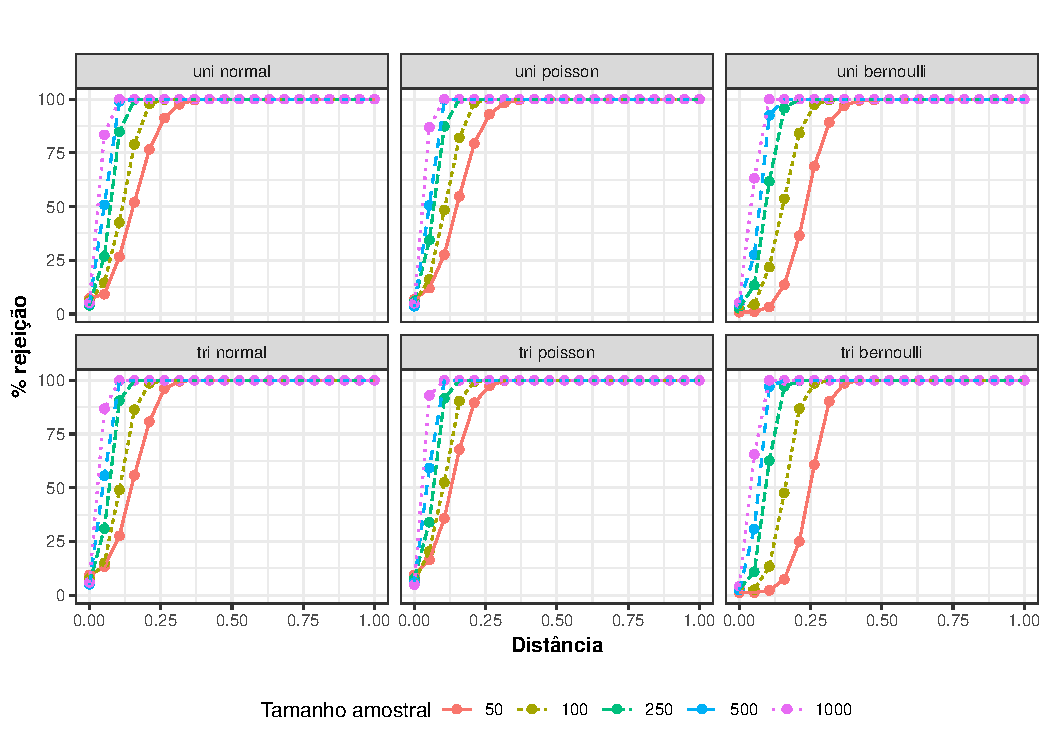
\includegraphics[width=15cm]{/home/lacf14/msc/4_dissertacao/5-simulacao/betas.pdf}
\end{figure}
\end{frame}

\begin{frame}{Parâmetros de regressão}
\protect\hypertarget{paruxe2metros-de-regressuxe3o-2}{}
\begin{itemize}
  \itemsep 2ex
  
  \item Quanto mais distante a hipótese é dos valores inicialmente simulados, maior é o percentual de rejeição. 
  
  \item Os menores percentuais foram observados na hipótese igual aos valores simulados. 
    \begin{itemize}
      \item \textbf{Univariados}: próximo de 5\% mesmo com tamanhos amostrais reduzidos. 
      \item \textbf{Trivariados}: não excedeu 10\% em tamanhos amostrais reduzidos. Próximo de 5\% em tamanhos amostrais iguais a 500.
    \end{itemize}

  \item Conforme aumenta-se o tamanho amostral, o percentual de rejeição aumenta para hipóteses pouco diferentes dos valores simulados dos parâmetros.

\end{itemize}
\end{frame}

\begin{frame}{Parâmetros de dispersão}
\protect\hypertarget{paruxe2metros-de-dispersuxe3o}{}
\beginAHalfColumnT
  \begin{itemize}
    \itemsep 2ex
    \item \textbf{Tamanhos amostrais}: 50, 100, 250, 500 e 1000.
  \item \textbf{500} conjuntos de dados.
  \item Cada unidade fornece 5 medidas ao conjunto de dados.
  \item Sem variáveis explicativas.
  \item Parâmetros de dispersão: $\tau_0 = 1$ e $\tau_1 = 0$.
\end{itemize}

\endColumns
\beginAHalfColumnT

\begin{itemize}
    \itemsep 2ex
    \item Parâmetros por distribuição:
    \begin{itemize}
        \item Normal: Média 5, desvio padrão 1.
        \item Poisson: Taxa igual a 10.
        \item Bernoulli: Probabilidade igual 0,6.
    \end{itemize}
  \end{itemize}
\endColumns
\end{frame}

\begin{frame}{Parâmetros de dispersão}
\protect\hypertarget{paruxe2metros-de-dispersuxe3o-1}{}
\begin{itemize}
  \itemsep 2ex
    \item Cenários \textbf{univariados} e \textbf{trivariados}.
    \item Para cada amostra gerada foi ajustado um McGLM.
  \item 20 diferentes hipóteses. 
    \begin{itemize}
      \item Decréscimo de 0,02 em $\tau_0$.
      \item Acréscimo de 0,02 em $\tau_1$.
    \end{itemize}

  \item Percentual de rejeição da hipótese nula por ponto. 

\end{itemize}
\end{frame}

\begin{frame}{}
\protect\hypertarget{section-1}{}
\begin{figure}[H]
\centering
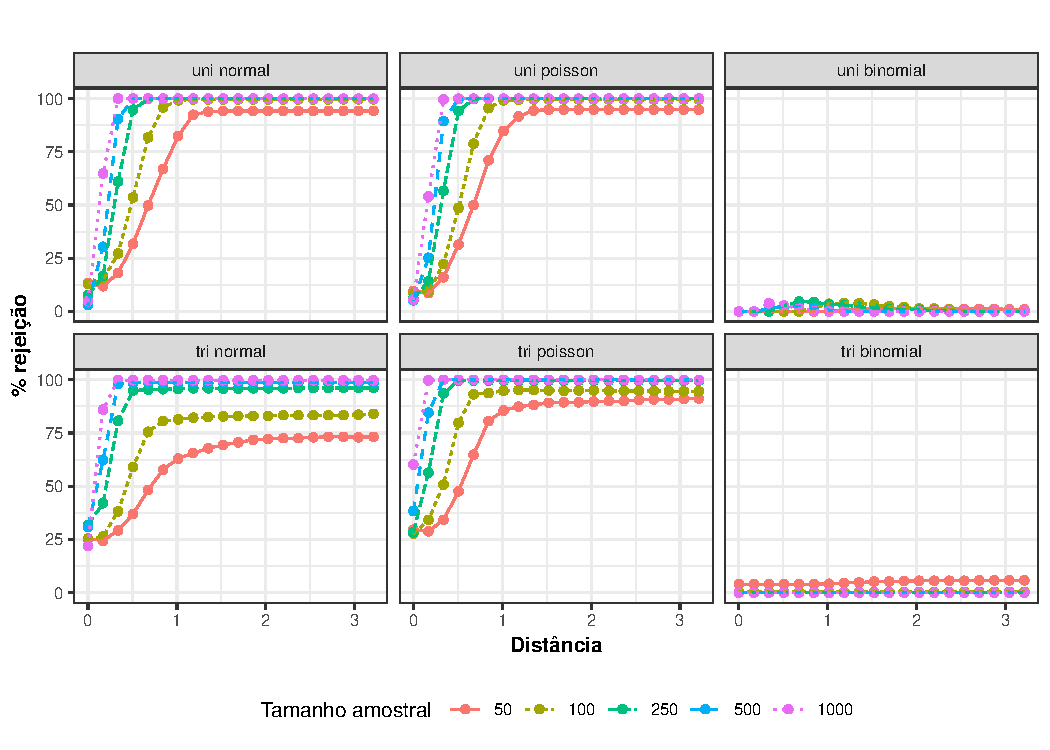
\includegraphics[width=15cm]{/home/lacf14/msc/4_dissertacao/5-simulacao/taus.pdf}
\end{figure}
\end{frame}

\begin{frame}{Parâmetros de dispersão}
\protect\hypertarget{paruxe2metros-de-dispersuxe3o-2}{}
\begin{itemize}
  \itemsep 2ex
  
  \item Quanto mais distante a hipótese é dos valores inicialmente simulados, maior é o percentual de rejeição. 
  
  \item Os menores percentuais foram observados na hipótese igual aos valores simulados. 
    \begin{itemize}
      \item \textbf{Univariados}: próximo de 8\% no menor tamanho amostal. Próximo de 5\% com tamanhos amostrais maiores que 250. 
      \item \textbf{Trivariados}: excede 10\% no menor tamanho amostal. Próximo de 7\% para tamanhos amostrais maiores.
    \end{itemize}

  \item Conforme aumenta-se o tamanho amostral, o percentual de rejeição aumenta para hipóteses pouco diferentes dos valores simulados dos parâmetros.

\end{itemize}
\end{frame}

\hypertarget{implementauxe7uxe3o-computacional}{%
\section{Implementação
computacional}\label{implementauxe7uxe3o-computacional}}

\begin{frame}{Implementação computacional}
\end{frame}

\begin{frame}{Implementação computacional}
\protect\hypertarget{implementauxe7uxe3o-computacional-1}{}
\begin{itemize}
  \itemsep 2ex
  
  \item \textbf{Implementar e disponibilizar} publicamente os testes apresentados.

  \item Complementar as já possíveis análises permitidas pelo pacote \emph{mcglm} \citep{mcglm}.

  \item O pacote \emph{htmcglm} já está disponível no \textbf{Comprehensive R Archive Network (CRAN)}.

  \item As funções implementadas geram resultados mostrando graus de liberdade e valores-p baseados no teste Wald aplicado a um McGLM.
\end{itemize}
\end{frame}

\begin{frame}{Implementação computacional}
\protect\hypertarget{implementauxe7uxe3o-computacional-2}{}
\begin{table}[h]
\centering
\begin{tabular}{ll}
\hline
Função                   & Descrição \\ 
\hline

mc\_anova\_I()           & ANOVA  tipo I \\
mc\_anova\_II()          & ANOVA  tipo II \\
mc\_anova\_III()         & ANOVA  tipo III \\

mc\_manova\_I()          & MANOVA tipo I \\
mc\_manova\_II()         & MANOVA tipo II \\
mc\_manova\_III()        & MANOVA tipo III \\

mc\_anova\_dispersion()        & ANOVA  tipo III para dispersão \\
mc\_manova\_dispersion()       & MANOVA tipo III para dispersão \\

mc\_multcomp()           & Testes de comparações múltiplas por resposta \\

mc\_mult\_multcomp()     & Testes de comparações múltiplas multivariado \\

mc\_linear\_hypothesis() & Hipóteses lineares gerais especificadas pelo usuário \\

\hline
\end{tabular}
\label{tab:funcoes}
\end{table}
\end{frame}

\hypertarget{anuxe1lise-de-dados}{%
\section{Análise de dados}\label{anuxe1lise-de-dados}}

\begin{frame}{Análise de dados}
\end{frame}

\begin{frame}{Análise de dados}
\protect\hypertarget{anuxe1lise-de-dados-1}{}
\begin{enumerate}
    \itemsep 2ex
  
  \item Contexto.
    
  \item Análise exploratória.
  
  \item Especificação do modelo.
  
  \item Resultados do ajuste.
  
  \item Testes de hipóteses.
 
\end{enumerate}
\end{frame}

\begin{frame}{Contexto}
\protect\hypertarget{contexto}{}
\begin{itemize}
  \itemsep 2ex
  
  \item Avaliar se o \textbf{uso de probióticos} é capaz de controlar \textbf{vício} e \textbf{transtorno da compulsão alimentar} em pacientes submetidos à \textbf{cirurgia bariátrica}.

  \item Conjunto de indivíduos divididos em 2 grupos: \textbf{placebo} ou \textbf{tratamento}.

  \item Indivíduos avaliados ao longo do tempo:
  \begin{itemize}
    \item \textbf{T0}: primeira avaliação, \textbf{antes} da cirurgia.
    \item \textbf{T1}: segunda avaliação, \textbf{3 meses} após a cirurgia.
    \item \textbf{T2}: terceira avaliação, \textbf{1 ano} após a cirurgia.
  \end{itemize}
\end{itemize}
\end{frame}

\begin{frame}{Contexto}
\protect\hypertarget{contexto-1}{}
\begin{itemize}
  \itemsep 2ex
  
  \item Avaliou-se os níveis de \textbf{vício} e \textbf{transtorno da compulsão alimentar} nos pacientes.

  \item Compulsão alimentar foi feita com base na \textbf{escala de compulsão alimentar (BES)}: escore, varia de 0 a 46.

  \item Vício alimentar foi utilizada a \textbf{escala de vício alimentar (YFAS)}: número de sintomas de vício, varia de 0 a 7.

  \item Para fins de análise, \textbf{YFAS} e \textbf{BES} foram transformados para a \textbf{escala unitária}, considerando que tratam-se de \textbf{variáveis restritas}.

\end{itemize}
\end{frame}

\begin{frame}{Contexto}
\protect\hypertarget{contexto-2}{}
\begin{itemize}
  \itemsep 2ex
  
  \item \textbf{71 indivíduos} (33 grupo placebo, 38 grupo tratamento). \textbf{184 observações}. 

  \item \textbf{Duas variáveis resposta}: BES e YFAS.

  \item As observações \textbf{não} são \textbf{independentes}.

  \item Técnicas de modelagem tradicionais seriam de difícil aplicação. 

  \item Cenário ideal para resolução via McGLM.

  \item Testes de hipóteses podem ser empregados para avaliar o efeito da interação entre momento e uso do probiótico sobre vício e compulsão alimentar.

\end{itemize}
\end{frame}

\begin{frame}{Contexto}
\protect\hypertarget{contexto-3}{}
Variáveis:

\begin{itemize}
  \item \textbf{id}: identificadora de indivíduo.
  \item \textbf{momento}: identificadora de momento (T0, T1, T2).
  \item \textbf{grupo}: identificadora de grupo (placebo, probiótico)
  \item \textbf{YFAS}: vício na escala unitária.
  \item \textbf{BES}: compulsão na escala unitária.
\end{itemize}
\end{frame}

\begin{frame}{Análise exploratória}
\protect\hypertarget{anuxe1lise-exploratuxf3ria}{}
\beginTwoThirdsColumn

\begin{figure}[H]
\centering
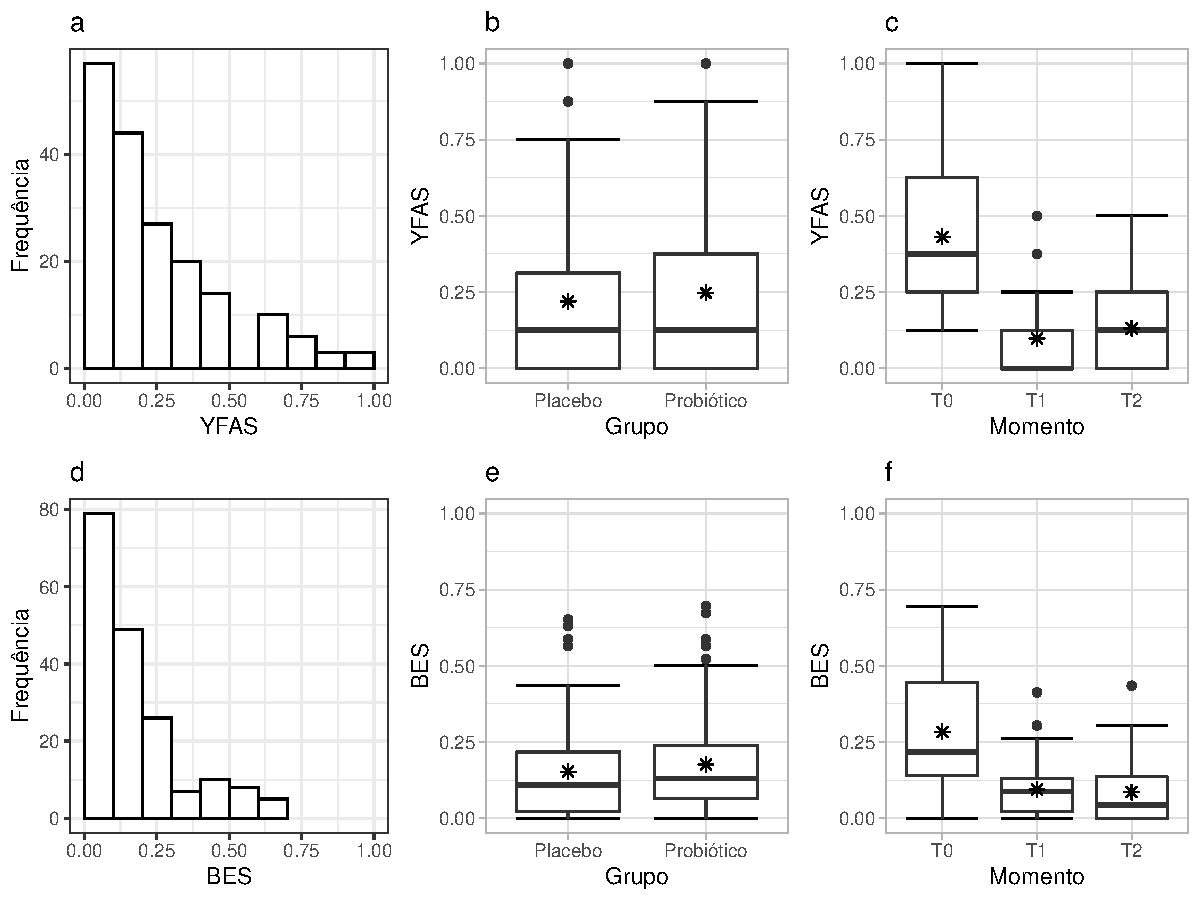
\includegraphics[width=10cm]{/home/lacf14/msc/4_dissertacao/7-aplicacao/descritiva.pdf}
\end{figure}

\endColumns\hfill
\beginAThirdColumn

\begin{figure}

{\centering 
\includegraphics[width=4cm]{defesa-lineu_files/figure-beamer/unnamed-chunk-3-1} 

}

\caption{Análise exploratória gráfica: (a) histograma YFAS, (b) boxplots YFAS em função de grupo, (c) boxplots YFAS em função de momento, (d) histograma BES, (b) boxplots BES em função de grupo, (c) boxplots BES em função de momento. O asterísco nos boxplots indica a média.}\label{fig:unnamed-chunk-3}
\end{figure}

\endColumns
\end{frame}

\begin{frame}{Análise exploratória}
\protect\hypertarget{anuxe1lise-exploratuxf3ria-1}{}
\begin{table}[H]
\centering
\begin{tabular}{ccccc}
\hline
\multirow{2}{*}{Grupo} & \multirow{2}{*}{Momento} & \multirow{2}{*}{n} & YFAS                  & BES                   \\ \cline{4-5} 
                       &                          &                    & Média (desvio padrão) & Média (desvio padrão) \\ \hline
Placebo                & T0                       & 33                 & 0,37 (0,26)           & 0,24 (0,20)           \\
Placebo                & T1                       & 32                 & 0,11 (0,15)           & 0,09 (0,10)           \\
Placebo                & T2                       & 22                 & 0,16 (0,15)           & 0,10 (0,12)           \\
Probiótico             & T0                       & 38                 & 0,49 (0,24)           & 0,32 (0,18)           \\
Probiótico             & T1                       & 37                 & 0,09 (0,12)           & 0,10 (0,08)           \\
Probiótico             & T2                       & 22                 & 0,10 (0,14)           & 0,07 (0,09)           \\ \hline
\end{tabular}
\caption{Número de indivíduos, média e desvio padrão para YFAS e BES para cada combinação de grupo e momento.}
\label{tab:descritiva1}
\end{table}
\end{frame}

\begin{frame}{Especificação do modelo}
\protect\hypertarget{especificauxe7uxe3o-do-modelo}{}
\begin{itemize}
  \itemsep 2ex
  
  \item Respostas foram transformadas para a \textbf{escala unitária}. 

  \item Função de ligação \textbf{logito}.

  \item Função de variância \textbf{binomial}. 

  \item Parâmetro de potência foram estimados.

  \item Foram consideradas categorias de referência o grupo placebo e o momento T0.

\end{itemize}
\end{frame}

\begin{frame}{Preditores lineares}
\protect\hypertarget{preditores-lineares}{}
\[
g_{r}(\mu_{r}) = \beta_{0r} + \beta_{1r} T1 + \beta_{2r} T2 + \beta_{3r} Probiotico + \beta_{4r} T1*Probiotico + \beta_{5r} T2*Probiotico
\]

\begin{itemize}
  \item $r$: variáveis respostas (1 para YFAS, 2 para BES). 
  \item $\beta_{0r}$: intercepto.
  \item $\beta_{1r}$: efeito do momento T1.
  \item $\beta_{2r}$: efeito do momento T2.
  \item $\beta_{3r}$: o efeito de probiótico. 
  \item $\beta_{4r}$: efeito da interação entre T1 e probiótico.
  \item $\beta_{5r}$: efeito da interação entre T2 e probiótico.
\end{itemize}
\end{frame}

\begin{frame}{Preditores matriciais}
\protect\hypertarget{preditores-matriciais}{}
\begin{itemize}
  \itemsep 2ex
  
  \item Iguais para ambas as respostas.

  \item A função $h(.)$ utilizada foi a identidade.

$$h\left \{ \boldsymbol{\Omega}(\boldsymbol{\tau}) \right \} = \tau_0Z_0 + \tau_1Z_1$$
  \begin{itemize}
    \item $\tau_0$ e $\tau_1$: parâmetros de dispersão. 
    \item $Z_0$: matriz identidade $184 \times 184$.
    \item $Z_1$: matriz $184 \times 184$ especificada de forma a explicitar que as \textbf{medidas provenientes do mesmo indivíduo são correlacionadas.} 
  \end{itemize}
\end{itemize}
\end{frame}

\begin{frame}{Análise de resíduos}
\protect\hypertarget{anuxe1lise-de-resuxedduos}{}
\begin{figure}[H]
\centering
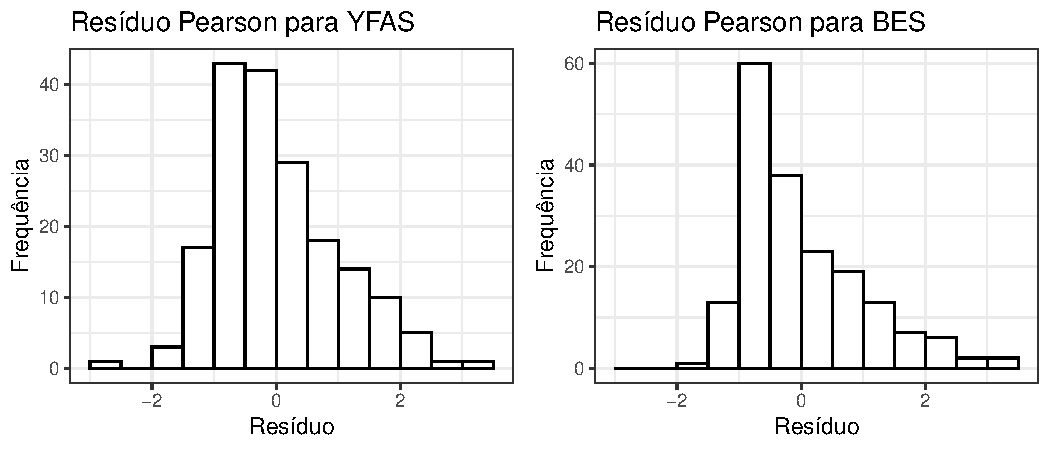
\includegraphics[width=15cm]{/home/lacf14/msc/4_dissertacao/7-aplicacao/res_hist.pdf}
\caption{Histograma dos resíduos de Pearson por resposta.}
\label{fig:diagnostico1}
\end{figure}
\end{frame}

\begin{frame}{Análise de resíduos}
\protect\hypertarget{anuxe1lise-de-resuxedduos-1}{}
\begin{figure}[H]
\centering
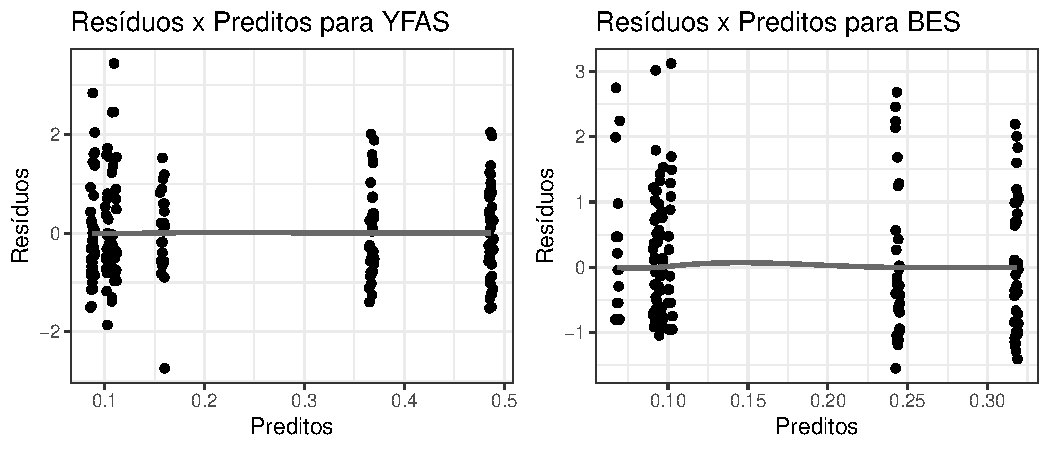
\includegraphics[width=15cm]{/home/lacf14/msc/4_dissertacao/7-aplicacao/res_pred.pdf}
\caption{Gráfico de resíduos Pearson versus preditos com linha de tendência suave para cada resposta.}
\label{fig:diagnostico2}
\end{figure}
\end{frame}

\begin{frame}{Análise de resíduos}
\protect\hypertarget{anuxe1lise-de-resuxedduos-2}{}
\begin{itemize}
  \itemsep 2ex
  
  \item Resíduos de Pearson para YFAS e BES apresentam \textbf{média 0} e \textbf{desvio padrão próximo de 1}. 

  \item Histogramas dos resíduos de Pearson: distribuição aproximadamente simétrica com a maior parte dos dados entre -2 e 2.

  \item Gráficos de resíduos versos preditos: mostram que não parece haver qualquer tipo de relação entre resíduos e preditos. 

  \item De forma geral, o modelo parece estar razoavelmente bem ajustado aos dados.
  
\end{itemize}
\end{frame}

\begin{frame}{Estimativas}
\protect\hypertarget{estimativas}{}
\begin{table}[]
\centering
\begin{tabular}{c|ccc|ccc}
\hline
\multirow{3}{*}{Parâmetro} & \multicolumn{3}{c|}{YFAS}                                              & \multicolumn{3}{c}{BES}                                                \\ \cline{2-7} 
                           & \multirow{2}{*}{Estimativa} & Intervalo de  & \multirow{2}{*}{Valor-p} & \multirow{2}{*}{Estimativa} & Intervalo de  & \multirow{2}{*}{Valor-p} \\
                           &                             & confiança     &                          &                             & confiança     &                          \\ \hline
$\beta_0$                  & -0,54                       & (-0,87;-0,22) & \textless{}0,01          & -1,13                       & (-1,44;-0,83) & \textless{}0,01          \\
$\beta_1$                  & -1,55                       & (-2,17;-0,94) & \textless{}0,01          & -1,16                       & (-1,62;-0,69) & \textless{}0,01          \\
$\beta_2$                  & -1,13                       & (-1,75;-0,51) & \textless{}0,01          & -1,05                       & (-1,58;-0,52) & \textless{}0,01          \\
$\beta_3$                  & 0,49                        & (0,05;0,93)   & 0,0284                   & 0,37                        & (-0,03;0,77)  & 0,0733                   \\
$\beta_4$                  & -0,73                       & (-1,60;0,14)  & 0,0                      & -0,33                       & (-0,96;0,30)  & 0,3081                   \\
$\beta_5$                  & -0,98                       & (-1,93;-0,03) & 0,0429                   & -0,80                       & (-1,58;-0,02) & 0,0449                   \\
$\tau_0$                   & 0,18                        & (0,01;0,35)   & 0,0411                   & 0,17                        & (0,00;0,34)   & 0,0458                   \\
$\tau_1$                   & 0,01                        & (-0,02;0,04)  & 0,5718                   & 0,04                        & (-0,01;0,10)  & 0,1357                   \\
$p$                        & 0,91                        & (0,47;1,34)   & \textless{}0,05          & 1,23                        & (0,77;1,68)   & \textless{}0,05          \\ \hline
\end{tabular}
\caption{Estimativas dos parâmetros, intervalos com 95\% de confiança e valores-p do modelo.}
\label{tab:my-table}
\end{table}
\end{frame}

\begin{frame}{Preditos}
\protect\hypertarget{preditos}{}
\begin{figure}[H]
\centering
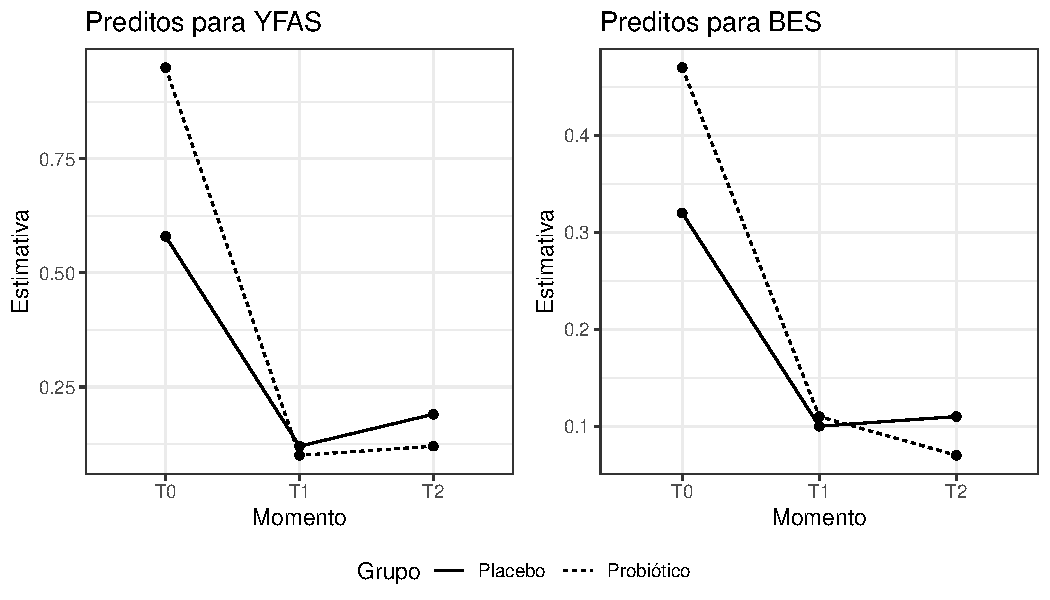
\includegraphics[width=13cm]{/home/lacf14/msc/4_dissertacao/7-aplicacao/fig_preditos.pdf}
\caption{Gráfico de preditos pelo modelo para cada combinação entre momento e grupo.}
\label{fig:preds}
\end{figure}
\end{frame}

\begin{frame}{Testes de hipóteses}
\protect\hypertarget{testes-de-hipuxf3teses-4}{}
\begin{itemize}
  \itemsep 2ex
  
  \item Até este ponto foi apresentada uma análise padrão. 

  \item Podemos fazer uso dos testes de hipóteses para explorar o modelo.
  
  \begin{itemize}
    \item Análise de variância multivariada do tipo II.
    \item Análise de variância univariada do tipo II.
    \item Comparações duas a duas entre momentos.
    \item Comparações entre grupos para cada momento.
    \item Análise da correlação de medidas tomadas em um mesmo indivíduo.
  \end{itemize}
  
\end{itemize}
\end{frame}

\begin{frame}{MANOVA tipo II}
\protect\hypertarget{manova-tipo-ii}{}
\begin{table}[H]
\centering
\begin{tabular}{cccc}
\hline
Variável      & Graus de liberdade & Qui-quadrado & Valor-p        \\ \hline
Intercepto    & 2                  & 53,1581      & \textless 0,01 \\
Momento       & 8                  & 139,0161     & \textless 0,01 \\
Grupo         & 6                  & 8,4928       & 0,2042         \\
Momento*Grupo & 4                  & 6,9923       & 0,1363         \\ \hline
\end{tabular}
\caption{Análise de variância multivariada do tipo II.}
\label{tab:manovaII}
\end{table}

Existência do efeito de momento e ausência de efeito de grupo.
\end{frame}

\begin{frame}{ANOVA tipo II}
\protect\hypertarget{anova-tipo-ii}{}
\begin{table}[H]
\centering
\begin{tabular}{c|c|cc|cc}
\hline
              &                    & \multicolumn{2}{c|}{YFAS}     & \multicolumn{2}{c}{BES}       \\ \hline
Variável      & GL & Qui-quadrado & Valor-p        & Qui-quadrado & Valor-p        \\ \hline
Intercepto    & 1                  & 10,6128      & \textless 0,01 & 53,1473      & \textless 0,01 \\
Momento       & 4                  & 102,9875     & \textless 0,01 & 99,5681      & \textless 0,01 \\
Grupo         & 3                  & 6,6837       & 0,0827         & 5,3083       & 0,1506         \\
Momento*Grupo & 2                  & 5,5984       & 0,0609         & 4,2477       & 0,1196         \\ \hline
\end{tabular}
\caption{Análise de variância univariada do tipo II.}
\label{tab:anovaII}
\end{table}

Existência do efeito de momento e ausência de efeito de grupo.
\end{frame}

\begin{frame}{Comparações múltiplas}
\protect\hypertarget{comparauxe7uxf5es-muxfaltiplas}{}
\begin{table}[H]
\centering
\begin{tabular}{cccc}
\hline
Contraste & Graus de liberdade & Qui-quadrado & Valor-p        \\ \hline
T0-T1     & 2                  & 97,9874      & \textless 0,01 \\
T0-T2     & 2                  & 67,2462      & \textless 0,01 \\
T1-T2     & 2                  & 2,4730       & 0,8712         \\ \hline
\end{tabular}
\caption{Comparações duas a duas entre momentos para ambas as respostas.}
\label{tab:mul-multcomp1}
\end{table}

\begin{itemize}
  \item $TO \neq T1$.
  \item $TO \neq T2$.
  \item $T1 = T2$.
\end{itemize}
\end{frame}

\begin{frame}{Comparações múltiplas}
\protect\hypertarget{comparauxe7uxf5es-muxfaltiplas-1}{}
\begin{table}[H]
\centering
\begin{tabular}{cccc}
\hline
Contraste                & Graus de liberdade & Qui-quadrado & Valor-p \\ \hline
T0:Placebo-T0:Probiótico & 2                  & 5,5819       & 0,9204  \\
T1:Placebo-T1:Probiótico & 2                  & 0,6096       & 1       \\
T2:Placebo-T2:Probiótico & 2                  & 1,7645       & 1       \\ \hline
\end{tabular}
\caption{Comparações duas a duas entre grupos para cada momento para ambas as respostas.}
\label{tab:mul-multcomp3}
\end{table}

Ausência de diferença entre grupos em cada momento.
\end{frame}

\begin{frame}{MANOVA para dispersão}
\protect\hypertarget{manova-para-dispersuxe3o}{}
\begin{table}[H]
\centering
\begin{tabular}{cccc}
\hline
Variável               & Graus de liberdade & Qui-quadrado & Valor-p        \\ \hline
$\tau_0$ & 2                  & 7,1936       & 0,0274 \\
$\tau_1$ & 2                  & 2,3201       & 0,3135         \\ \hline
\end{tabular}
\caption{Análise de variância multivariada do tipo III para parâmetros de dispersão.}
\label{tab:manova_disp}
\end{table}

Não há evidência para crer que as medidas tomadas em um mesmo indivíduo
apresentam correlação.
\end{frame}

\hypertarget{considerauxe7uxf5es-finais}{%
\section{Considerações finais}\label{considerauxe7uxf5es-finais}}

\begin{frame}{Considerações finais}
\end{frame}

\begin{frame}{Considerações finais}
\protect\hypertarget{considerauxe7uxf5es-finais-1}{}
\begin{itemize}
  \itemsep 2ex
  
  \item Objetivo: teste \textbf{Wald} em \textbf{McGLMs}. 
  \item Chegamos a procedimentos para:
  \begin{itemize}
    \item \textbf{Testes de hipóteses lineares gerais}.
    \item \textbf{ANOVA}.
    \item \textbf{MANOVA}.
    \item \textbf{Testes de comparações múltiplas}. 
  \end{itemize}
  
  \item \textbf{Proposta implementada} na biblioteca R \emph{htmcglm}, complementa a biblioteca \emph{mcglm}.

\end{itemize}
\end{frame}

\begin{frame}{Conclusões gerais}
\protect\hypertarget{conclusuxf5es-gerais}{}
\begin{itemize}
  \itemsep 2ex
  
  \item As propriedades dos testes foram avaliadas com base em \textbf{estudos de simulação}.

  \item Os estudos de simulação mostraram que:

  \begin{itemize}
    \itemsep 2ex
      \item Quanto mais distante a hipótese é dos valores inicialmente simulados, maior é o percentual de rejeição. 
      \item Os menores percentuais foram observados na hipótese igual aos valores simulados.
      \item Conforme aumenta-se o tamanho amostral, o percentual de rejeição aumenta para hipóteses pouco diferentes dos valores simulados dos parâmetros.
  \end{itemize}
\end{itemize}
\end{frame}

\begin{frame}{Conclusões gerais}
\protect\hypertarget{conclusuxf5es-gerais-1}{}
\begin{itemize}
  \itemsep 2ex
  
  \item Aplicação: efeito do uso de \textbf{probióticos} no controle de \textbf{vícios e compulsões alimentares}.

  \item Os resultados, baseados nos testes propostos indicam que: 
  \begin{itemize}
    \item Existe efeito de momento.
    \item Existem diferenças entre o primeiro versus segundo e primeiro versus terceiro momento, mas os dois últimos momentos não diferem entre si.
    \item Ausência de diferença entre grupos em cada momento.
    \item Não há evidência para crer que as medidas tomadas em um mesmo indivíduo apresentam correlação.
  \end{itemize}
\end{itemize}
\end{frame}

\begin{frame}{Limitações}
\protect\hypertarget{limitauxe7uxf5es}{}
Casos não explorados nos estudos de simulação, tais como:

\begin{itemize}
  \itemsep 2ex
  
  \item Desempenho dos testes ao definir hipóteses lineares que combinem \textbf{parâmetros de diferentes tipos}.
  \item Impacto de um \textbf{número diferente de observações} por indivíduos em problemas longitudinais ou de medidas repetidas. 
  \item Impacto no poder do teste conforme o \textbf{número de parâmetros testados} aumenta.
  \item Comportamento do teste em problemas multivariados com \textbf{distribuições de probabilidade diferentes} das exploradas.

\end{itemize}
\end{frame}

\begin{frame}{Trabalhos futuros}
\protect\hypertarget{trabalhos-futuros}{}
Avaliação de parâmetros de McGLMs para um melhor entendimento do impacto
dos elementos em problemas de modelagem.

Algumas possibilidades são:

\begin{itemize}
  \item Correções de valores-p de acordo com o tamanho das hipóteses testadas. 
  \item Procedimentos além do teste Wald (como o teste Escore e o teste da razão de verossimilhanças). 
  \item Outros procedimentos para comparações múltiplas. 
  \item Lidar com contrastes alternativos aos usuais. 
  \item Explorar procedimentos para seleção covariáveis.
\end{itemize}
\end{frame}

\begin{frame}{}
\protect\hypertarget{section-2}{}
\begin{center}

  {\huge \href{https://lineu96.github.io/st/}{Obrigado!}}
  
  \vspace{0.5cm}
    
  {\normalsize \href{https://lineu96.github.io/st/}{Lineu Alberto Cavazani de Freitas}}
  
  {\normalsize \href{https://lineu96.github.io/st/}{lineuacf@gmail.com}}
  
  {\normalsize \href{https://lineu96.github.io/st/}{https://lineu96.github.io/st/}}
  
  {\normalsize \href{http://www.prppg.ufpr.br/ppginformatica/?lang=pb}{PPG Informática}}

\end{center}

\begin{center}
  
\includegraphics[height=1.8cm]{config/capes_tp2.png}\hspace{2em}
  
\includegraphics[height=1.8cm]{config/ufpr-transparent-600px.png}\hspace{2em}
  
\includegraphics[height=1.8cm]{config/dsbd-2x2-trans.png}
\end{center}
\end{frame}

\begin{frame}[allowframebreaks]{}
  \bibliographytrue
  \bibliography{config/referencias.bib}
\end{frame}

\end{document}
